% Contact author: frank.nielsen.x@gmail.com
% IT-21-0862
% On $f$-divergences between Cauchy distributions

%% bare_jrnl.tex
%% V1.4b
%% 2015/08/26
%% by Michael Shell
%% see http://www.michaelshell.org/
%% for current contact information.
%%
%% This is a skeleton file demonstrating the use of IEEEtran.cls
%% (requires IEEEtran.cls version 1.8b or later) with an IEEE
%% journal paper.
%%
%% Support sites:
%% http://www.michaelshell.org/tex/ieeetran/
%% http://www.ctan.org/pkg/ieeetran
%% and
%% http://www.ieee.org/

%%*************************************************************************
%% Legal Notice:
%% This code is offered as-is without any warranty either expressed or
%% implied; without even the implied warranty of MERCHANTABILITY or
%% FITNESS FOR A PARTICULAR PURPOSE! 
%% User assumes all risk.
%% In no event shall the IEEE or any contributor to this code be liable for
%% any damages or losses, including, but not limited to, incidental,
%% consequential, or any other damages, resulting from the use or misuse
%% of any information contained here.
%%
%% All comments are the opinions of their respective authors and are not
%% necessarily endorsed by the IEEE.
%%
%% This work is distributed under the LaTeX Project Public License (LPPL)
%% ( http://www.latex-project.org/ ) version 1.3, and may be freely used,
%% distributed and modified. A copy of the LPPL, version 1.3, is included
%% in the base LaTeX documentation of all distributions of LaTeX released
%% 2003/12/01 or later.
%% Retain all contribution notices and credits.
%% ** Modified files should be clearly indicated as such, including  **
%% ** renaming them and changing author support contact information. **
%%*************************************************************************


% *** Authors should verify (and, if needed, correct) their LaTeX system  ***
% *** with the testflow diagnostic prior to trusting their LaTeX platform ***
% *** with production work. The IEEE's font choices and paper sizes can   ***
% *** trigger bugs that do not appear when using other class files.       ***                          ***
% The testflow support page is at:
% http://www.michaelshell.org/tex/testflow/



\documentclass[journal]{IEEEtran}
%
% If IEEEtran.cls has not been installed into the LaTeX system files,
% manually specify the path to it like:
% \documentclass[journal]{../sty/IEEEtran}





% Some very useful LaTeX packages include:
% (uncomment the ones you want to load)


% *** MISC UTILITY PACKAGES ***
%
%\usepackage{ifpdf}
% Heiko Oberdiek's ifpdf.sty is very useful if you need conditional
% compilation based on whether the output is pdf or dvi.
% usage:
% \ifpdf
%   % pdf code
% \else
%   % dvi code
% \fi
% The latest version of ifpdf.sty can be obtained from:
% http://www.ctan.org/pkg/ifpdf
% Also, note that IEEEtran.cls V1.7 and later provides a builtin
% \ifCLASSINFOpdf conditional that works the same way.
% When switching from latex to pdflatex and vice-versa, the compiler may
% have to be run twice to clear warning/error messages.






% *** CITATION PACKAGES ***
%
%\usepackage{cite}
% cite.sty was written by Donald Arseneau
% V1.6 and later of IEEEtran pre-defines the format of the cite.sty package
% \cite{} output to follow that of the IEEE. Loading the cite package will
% result in citation numbers being automatically sorted and properly
% "compressed/ranged". e.g., [1], [9], [2], [7], [5], [6] without using
% cite.sty will become [1], [2], [5]--[7], [9] using cite.sty. cite.sty's
% \cite will automatically add leading space, if needed. Use cite.sty's
% noadjust option (cite.sty V3.8 and later) if you want to turn this off
% such as if a citation ever needs to be enclosed in parenthesis.
% cite.sty is already installed on most LaTeX systems. Be sure and use
% version 5.0 (2009-03-20) and later if using hyperref.sty.
% The latest version can be obtained at:
% http://www.ctan.org/pkg/cite
% The documentation is contained in the cite.sty file itself.






% *** GRAPHICS RELATED PACKAGES ***
%
\ifCLASSINFOpdf
  % \usepackage[pdftex]{graphicx}
  % declare the path(s) where your graphic files are
  % \graphicspath{{../pdf/}{../jpeg/}}
  % and their extensions so you won't have to specify these with
  % every instance of \includegraphics
  % \DeclareGraphicsExtensions{.pdf,.jpeg,.png}
\else
  % or other class option (dvipsone, dvipdf, if not using dvips). graphicx
  % will default to the driver specified in the system graphics.cfg if no
  % driver is specified.
  % \usepackage[dvips]{graphicx}
  % declare the path(s) where your graphic files are
  % \graphicspath{{../eps/}}
  % and their extensions so you won't have to specify these with
  % every instance of \includegraphics
  % \DeclareGraphicsExtensions{.eps}
\fi
% graphicx was written by David Carlisle and Sebastian Rahtz. It is
% required if you want graphics, photos, etc. graphicx.sty is already
% installed on most LaTeX systems. The latest version and documentation
% can be obtained at: 
% http://www.ctan.org/pkg/graphicx
% Another good source of documentation is "Using Imported Graphics in
% LaTeX2e" by Keith Reckdahl which can be found at:
% http://www.ctan.org/pkg/epslatex
%
% latex, and pdflatex in dvi mode, support graphics in encapsulated
% postscript (.eps) format. pdflatex in pdf mode supports graphics
% in .pdf, .jpeg, .png and .mps (metapost) formats. Users should ensure
% that all non-photo figures use a vector format (.eps, .pdf, .mps) and
% not a bitmapped formats (.jpeg, .png). The IEEE frowns on bitmapped formats
% which can result in "jaggedy"/blurry rendering of lines and letters as
% well as large increases in file sizes.
%
% You can find documentation about the pdfTeX application at:
% http://www.tug.org/applications/pdftex


\usepackage{tikz} 
\usepackage{tikz-cd} 
\usetikzlibrary{positioning} 

\usepackage{amsmath,amsthm,amssymb,amsfonts,empheq}
\usepackage{orcidlink}
\usepackage[hidelinks]{hyperref}
\usepackage{cleveref}

\newtheorem{theorem}{Theorem}
\newtheorem{lemma}[theorem]{Lemma}
\newtheorem{corollary}[theorem]{Corollary}
\newtheorem{proposition}[theorem]{Proposition}
\newtheorem{definition}[theorem]{Definition}
\newtheorem{remark}[theorem]{Remark} 
\newtheorem{assumption}[theorem]{Assumption} 
\newtheorem{problem}[theorem]{Problem} 



\def\leftsup#1{{}^{#1}}
\def\calLC{\mathcal{LC}}
\def\lc{\mathrm{lc}}
\def\wc{\mathrm{wc}}
\def\HM{\mathrm{HM}}
\def\JS{\mathrm{JS}}
\def\TV{\mathrm{TV}}
\def\LC{\mathrm{LC}}
\def\BC{\mathrm{BC}}
\def\Bhat{\mathrm{Bhat}}
\def\dz{\mathrm{d}z}
\def\Im{\mathrm{Im}}
\def\Re{\mathrm{Re}}
\def\FR{\mathrm{FR}}
\def\SL{\mathrm{SL}}
\def\SU{\mathrm{SU}}
\def\KC{\mathrm{KC}}
\def\bbC{\mathbb{C}}
\def\bbU{\mathbb{U}}
\def\bbD{\mathbb{D}}
\def\calLN{\mathcal{LN}}
\def\calG{\mathcal{G}}
\def\calL{\mathcal{L}}
\def\calH{\mathcal{H}}
\def\GL{\mathrm{GL}}
\def\arccosh{\mathrm{arccosh}}
\def\sech{\mathrm{sech}}
\def\dl{\mathrm{d}l}
\def\ds{\mathrm{d}s}
\def\dlambda{\mathrm{d}\lambda}
\def\dtheta{\mathrm{d}\theta}
\def\JS{\mathrm{JS}}
\def\MI{\mathrm{MI}}
\def\elliptical{\mathrm{ell}}
\def\calM{\mathcal{M}}
\def\normal{\mathcal{N}}
\def\Rayleigh{\mathrm{Rayleigh}}
\def\Cauchy{\mathrm{Cauchy}}
\def\Mah{\mathrm{Mah}}
\def\IS{\mathrm{IS}}
\def\diag{\mathrm{diag}}
\def\calE{\mathcal{E}}
\def\calR{\mathcal{R}}
\def\calL{\mathcal{L}}
\def\calN{\mathcal{N}}
\def\calC{\mathcal{C}}
\def\calS{\mathcal{S}}
\def\calK{\mathcal{K}}
\def\calP{\mathcal{P}}
\def\calQ{\mathcal{Q}}
\def\LS{\mathrm{LS}}
\def\tr{\mathrm{tr}}	
\def\bbP{\mathbb{P}}
\def\eqdef{:=}
\def\hcross{{h^\times}}
\def\hcrossent#1#2{{\hcross}\left(#1:#2\right)}
\def\arctanh{\mathrm{arctanh}}
\def\dmu{\mathrm{d}\mu}
\def\bbH{\mathbb{H}}
\def\dx{\mathrm{d}x}
\def\dy{\mathrm{d}y}
\def\KL{\mathrm{KL}}
\def\kl{\mathrm{kl}}
\def\bbR{{\mathbb{R}}}
\def\calF{\mathcal{F}}
\def\calX{\mathcal{X}}
\def\calY{\mathcal{Y}}
\def\st{\ :\ }
\def\SO{\mathrm{SO}}
\def\Jac{\mathrm{Jac}}
\def\equaldist{\stackrel{d}{=}}
\def\bbG{\mathbb{G}}
\def\mattwotwo#1#2#3#4{\left[\begin{array}{cc}#1 & #2\\ #3 & #4\end{array}\right]}
\def\Sym{\mathrm{Sym}}
\def\cc{\mathrm{cc}}
\def\Cauchy{\mathrm{Cauchy}}
\def\CCauchy{\mathrm{CCauchy}}
\def\WCauchy{\mathrm{WCauchy}}
\def\LogCauchy{\mathrm{LogCauchy}}

% *** MATH PACKAGES ***
%
%\usepackage{amsmath}
% A popular package from the American Mathematical Society that provides
% many useful and powerful commands for dealing with mathematics.
%
% Note that the amsmath package sets \interdisplaylinepenalty to 10000
% thus preventing page breaks from occurring within multiline equations. Use:
\interdisplaylinepenalty=2500
% after loading amsmath to restore such page breaks as IEEEtran.cls normally
% does. amsmath.sty is already installed on most LaTeX systems. The latest
% version and documentation can be obtained at:
% http://www.ctan.org/pkg/amsmath





% *** SPECIALIZED LIST PACKAGES ***
%
%\usepackage{algorithmic}
% algorithmic.sty was written by Peter Williams and Rogerio Brito.
% This package provides an algorithmic environment fo describing algorithms.
% You can use the algorithmic environment in-text or within a figure
% environment to provide for a floating algorithm. Do NOT use the algorithm
% floating environment provided by algorithm.sty (by the same authors) or
% algorithm2e.sty (by Christophe Fiorio) as the IEEE does not use dedicated
% algorithm float types and packages that provide these will not provide
% correct IEEE style captions. The latest version and documentation of
% algorithmic.sty can be obtained at:
% http://www.ctan.org/pkg/algorithms
% Also of interest may be the (relatively newer and more customizable)
% algorithmicx.sty package by Szasz Janos:
% http://www.ctan.org/pkg/algorithmicx




% *** ALIGNMENT PACKAGES ***
%
%\usepackage{array}
% Frank Mittelbach's and David Carlisle's array.sty patches and improves
% the standard LaTeX2e array and tabular environments to provide better
% appearance and additional user controls. As the default LaTeX2e table
% generation code is lacking to the point of almost being broken with
% respect to the quality of the end results, all users are strongly
% advised to use an enhanced (at the very least that provided by array.sty)
% set of table tools. array.sty is already installed on most systems. The
% latest version and documentation can be obtained at:
% http://www.ctan.org/pkg/array


% IEEEtran contains the IEEEeqnarray family of commands that can be used to
% generate multiline equations as well as matrices, tables, etc., of high
% quality.




% *** SUBFIGURE PACKAGES ***
%\ifCLASSOPTIONcompsoc
%  \usepackage[caption=false,font=normalsize,labelfont=sf,textfont=sf]{subfig}
%\else
%  \usepackage[caption=false,font=footnotesize]{subfig}
%\fi
% subfig.sty, written by Steven Douglas Cochran, is the modern replacement
% for subfigure.sty, the latter of which is no longer maintained and is
% incompatible with some LaTeX packages including fixltx2e. However,
% subfig.sty requires and automatically loads Axel Sommerfeldt's caption.sty
% which will override IEEEtran.cls' handling of captions and this will result
% in non-IEEE style figure/table captions. To prevent this problem, be sure
% and invoke subfig.sty's "caption=false" package option (available since
% subfig.sty version 1.3, 2005/06/28) as this is will preserve IEEEtran.cls
% handling of captions.
% Note that the Computer Society format requires a larger sans serif font
% than the serif footnote size font used in traditional IEEE formatting
% and thus the need to invoke different subfig.sty package options depending
% on whether compsoc mode has been enabled.
%
% The latest version and documentation of subfig.sty can be obtained at:
% http://www.ctan.org/pkg/subfig




% *** FLOAT PACKAGES ***
%
%\usepackage{fixltx2e}
% fixltx2e, the successor to the earlier fix2col.sty, was written by
% Frank Mittelbach and David Carlisle. This package corrects a few problems
% in the LaTeX2e kernel, the most notable of which is that in current
% LaTeX2e releases, the ordering of single and double column floats is not
% guaranteed to be preserved. Thus, an unpatched LaTeX2e can allow a
% single column figure to be placed prior to an earlier double column
% figure.
% Be aware that LaTeX2e kernels dated 2015 and later have fixltx2e.sty's
% corrections already built into the system in which case a warning will
% be issued if an attempt is made to load fixltx2e.sty as it is no longer
% needed.
% The latest version and documentation can be found at:
% http://www.ctan.org/pkg/fixltx2e


%\usepackage{stfloats}
% stfloats.sty was written by Sigitas Tolusis. This package gives LaTeX2e
% the ability to do double column floats at the bottom of the page as well
% as the top. (e.g., "\begin{figure*}[!b]" is not normally possible in
% LaTeX2e). It also provides a command:
%\fnbelowfloat
% to enable the placement of footnotes below bottom floats (the standard
% LaTeX2e kernel puts them above bottom floats). This is an invasive package
% which rewrites many portions of the LaTeX2e float routines. It may not work
% with other packages that modify the LaTeX2e float routines. The latest
% version and documentation can be obtained at:
% http://www.ctan.org/pkg/stfloats
% Do not use the stfloats baselinefloat ability as the IEEE does not allow
% \baselineskip to stretch. Authors submitting work to the IEEE should note
% that the IEEE rarely uses double column equations and that authors should try
% to avoid such use. Do not be tempted to use the cuted.sty or midfloat.sty
% packages (also by Sigitas Tolusis) as the IEEE does not format its papers in
% such ways.
% Do not attempt to use stfloats with fixltx2e as they are incompatible.
% Instead, use Morten Hogholm'a dblfloatfix which combines the features
% of both fixltx2e and stfloats:
%
% \usepackage{dblfloatfix}
% The latest version can be found at:
% http://www.ctan.org/pkg/dblfloatfix




%\ifCLASSOPTIONcaptionsoff
%  \usepackage[nomarkers]{endfloat}
% \let\MYoriglatexcaption\caption
% \renewcommand{\caption}[2][\relax]{\MYoriglatexcaption[#2]{#2}}
%\fi
% endfloat.sty was written by James Darrell McCauley, Jeff Goldberg and 
% Axel Sommerfeldt. This package may be useful when used in conjunction with 
% IEEEtran.cls'  captionsoff option. Some IEEE journals/societies require that
% submissions have lists of figures/tables at the end of the paper and that
% figures/tables without any captions are placed on a page by themselves at
% the end of the document. If needed, the draftcls IEEEtran class option or
% \CLASSINPUTbaselinestretch interface can be used to increase the line
% spacing as well. Be sure and use the nomarkers option of endfloat to
% prevent endfloat from "marking" where the figures would have been placed
% in the text. The two hack lines of code above are a slight modification of
% that suggested by in the endfloat docs (section 8.4.1) to ensure that
% the full captions always appear in the list of figures/tables - even if
% the user used the short optional argument of \caption[]{}.
% IEEE papers do not typically make use of \caption[]'s optional argument,
% so this should not be an issue. A similar trick can be used to disable
% captions of packages such as subfig.sty that lack options to turn off
% the subcaptions:
% For subfig.sty:
% \let\MYorigsubfloat\subfloat
% \renewcommand{\subfloat}[2][\relax]{\MYorigsubfloat[]{#2}}
% However, the above trick will not work if both optional arguments of
% the \subfloat command are used. Furthermore, there needs to be a
% description of each subfigure *somewhere* and endfloat does not add
% subfigure captions to its list of figures. Thus, the best approach is to
% avoid the use of subfigure captions (many IEEE journals avoid them anyway)
% and instead reference/explain all the subfigures within the main caption.
% The latest version of endfloat.sty and its documentation can obtained at:
% http://www.ctan.org/pkg/endfloat
%
% The IEEEtran \ifCLASSOPTIONcaptionsoff conditional can also be used
% later in the document, say, to conditionally put the References on a 
% page by themselves.




% *** PDF, URL AND HYPERLINK PACKAGES ***
%
\usepackage{url}
% url.sty was written by Donald Arseneau. It provides better support for
% handling and breaking URLs. url.sty is already installed on most LaTeX
% systems. The latest version and documentation can be obtained at:
% http://www.ctan.org/pkg/url
% Basically, \url{my_url_here}.




% *** Do not adjust lengths that control margins, column widths, etc. ***
% *** Do not use packages that alter fonts (such as pslatex).         ***
% There should be no need to do such things with IEEEtran.cls V1.6 and later.
% (Unless specifically asked to do so by the journal or conference you plan
% to submit to, of course. )


% correct bad hyphenation here
%\hyphenation{op-tical net-works semi-conduc-tor}


\begin{document}
%
% paper title
% Titles are generally capitalized except for words such as a, an, and, as,
% at, but, by, for, in, nor, of, on, or, the, to and up, which are usually
% not capitalized unless they are the first or last word of the title.
% Linebreaks \\ can be used within to get better formatting as desired.
% Do not put math or special symbols in the title.
\title{On $f$-divergences between Cauchy distributions\thanks{This paper was presented in part in the Geometric Science of Information (2021), Lecture Notes in Computer Science, Volume 12829, pages 799--807, Springer 2021.}}
%
%
% author names and IEEE memberships
% note positions of commas and nonbreaking spaces ( ~ ) LaTeX will not break
% a structure at a ~ so this keeps an author's name from being broken across
% two lines.
% use \thanks{} to gain access to the first footnote area
% a separate \thanks must be used for each paragraph as LaTeX2e's \thanks
% was not built to handle multiple paragraphs
%

\author{Frank~Nielsen\textsuperscript{\orcidlink{0000-0001-5728-0726}}\,,~\IEEEmembership{Senior Member,~IEEE,}
Kazuki Okamura \textsuperscript{\orcidlink{0000-0003-4467-4165}}\,,~\IEEEmembership{Non-Member}

\thanks{Manuscript received on xxx 
(\emph{Corresponding author: Frank Nielsen.})}
\thanks{Frank Nielsen is with
Sony Computer Science Laboratories, Inc., Japan (e-mail: \texttt{Frank.Nielsen@acm.org})}
\thanks{Kazuki Okamura is with
Department of Mathematics, Faculty of Science, Shizuoka University, Japan
(e-mail: \texttt{okamura.kazuki@shizuoka.ac.jp}). He was supported by JSPS KAKENHI 19K14549.}}

%\author{Michael~Shell,~\IEEEmembership{Member,~IEEE,}
%        John~Doe,~\IEEEmembership{Fellow,~OSA,}
%       and~Jane~Doe,~\IEEEmembership{Life~Fellow,~IEEE}% <-this % stops a space
%\thanks{M. Shell was with the Department
%of Electrical and Computer Engineering, Georgia Institute of Technology, Atlanta,
%GA, 30332 USA e-mail: (see http://www.michaelshell.org/contact.html).}% <-this % stops a space
%\thanks{J. Doe and J. Doe are with Anonymous University.}% <-this % stops a space
%\thanks{Manuscript received April 19, 2005; revised August 26, 2015.}}

% note the % following the last \IEEEmembership and also \thanks - 
% these prevent an unwanted space from occurring between the last author name
% and the end of the author line. i.e., if you had this:
% 
% \author{....lastname \thanks{...} \thanks{...} }
%                     ^------------^------------^----Do not want these spaces!
%
% a space would be appended to the last name and could cause every name on that
% line to be shifted left slightly. This is one of those "LaTeX things". For
% instance, "\textbf{A} \textbf{B}" will typeset as "A B" not "AB". To get
% "AB" then you have to do: "\textbf{A}\textbf{B}"
% \thanks is no different in this regard, so shield the last } of each \thanks
% that ends a line with a % and do not let a space in before the next \thanks.
% Spaces after \IEEEmembership other than the last one are OK (and needed) as
% you are supposed to have spaces between the names. For what it is worth,
% this is a minor point as most people would not even notice if the said evil
% space somehow managed to creep in.



% The paper headers
%\markboth{Journal of \LaTeX\ Class Files,~Vol.~14, No.~8, August~2015}%
%{Shell \MakeLowercase{\textit{et al.}}: Bare Demo of IEEEtran.cls for IEEE Journals}
% The only time the second header will appear is for the odd numbered pages
% after the title page when using the twoside option.
% 
% *** Note that you probably will NOT want to include the author's ***
% *** name in the headers of peer review papers.                   ***
% You can use \ifCLASSOPTIONpeerreview for conditional compilation here if
% you desire.




% If you want to put a publisher's ID mark on the page you can do it like
% this:
%\IEEEpubid{0000--0000/00\$00.00~\copyright~2015 IEEE}
% Remember, if you use this you must call \IEEEpubidadjcol in the second
% column for its text to clear the IEEEpubid mark.



% use for special paper notices
%\IEEEspecialpapernotice{(Invited Paper)}




% make the title area
\maketitle

% As a general rule, do not put math, special symbols or citations
% in the abstract or keywords.
\begin{abstract}
We prove that all $f$-divergences between univariate Cauchy distributions are symmetric.
Furthermore, those $f$-divergences can be calculated as strictly increasing scalar functions of the chi-square divergence. 
We report a criterion which allows one to expand $f$-divergences as converging series of power chi divergences, and exemplifies the technique for some $f$-divergences between Cauchy distributions.
In contrast with the univariate case, we show that the $f$-divergences between multivariate Cauchy densities are in general asymmetric although symmetric when the Cauchy scale matrices coincide. 
Then we prove that the square roots of the Kullback-Leibler and Bhattacharyya divergences between univariate Cauchy distributions yield complete metric spaces. 
Finally, we show that the square root of the Kullback-Leibler divergence between univariate Cauchy distributions can be isometrically embedded into a Hilbert space.
\end{abstract}

% Note that keywords are not normally used for peerreview papers.
\begin{IEEEkeywords}
Cauchy distributions; Location-scale families; $f$-divergences; Complex analysis; maximal invariant; M\"obius transformations; conditionally negative-definite kernel.  
%IEEE, IEEEtran, journal, \LaTeX, paper, template.
\end{IEEEkeywords}






% For peer review papers, you can put extra information on the cover
% page as needed:
% \ifCLASSOPTIONpeerreview
% \begin{center} \bfseries EDICS Category: 3-BBND \end{center}
% \fi
%
% For peerreview papers, this IEEEtran command inserts a page break and
% creates the second title. It will be ignored for other modes.
\IEEEpeerreviewmaketitle



\section{Introduction}


The probability density function $p_{l,s}(x)$ of a random variable $X$ following a Cauchy distribution $\Cauchy(l,s)$~\cite{mccullagh1992conditional} is
$$
p_{l,s}(x) := \frac{s}{\pi (s^2+(x-l)^2)},\quad x\in\bbR.
$$
Parameter $l\in\bbR$ characterizes the median and parameter $s>0$ is called the probable error~\cite{mccullagh1992conditional}.
The set of Cauchy distributions forms a location-scale family~\cite{KassVos-2011}: 
$$
\calC=\left\{p_{l,s}(x)=\frac{1}{s} p\left(\frac{x-l}{s}\right) \st (l,s)\in \bbR\times\bbR_{++}\right\},
$$ 
where $p(x)$ denotes the Cauchy standard density and $\bbR_{++}$ denotes  the set of positive real numbers:
\begin{equation}\label{eq:stdcauchy}
p(x):=\frac{1}{\pi(1+x^2)}.
\end{equation}
Thus parameters $l\in\bbR$ and $s>0$ denote the location parameter and the scale parameter of the Cauchy distribution, respectively. 
The Cauchy distributions belong to two larger families of distributions: 
Namely, the $t$-Student distributions (for $\nu=1$ degrees of freedom) and the $q$-normal distributions~\cite{naudts2011generalised} (for $q=2$).
In Physics, the Cauchy distributions are also sometimes called the Lorentzian distributions~\cite{filipovic2012two} or the Breit–Wigner distribution~\cite{vsirca2016special}. 


In information theory, the Cauchy distributions have been used to model and analyze severe non-Gaussian noise with infinite variance ~(\cite{miller1972detectors,sousa1992performance,merhav2011optimum})  modeling so-called Cauchy channels in~\cite{fahs2014cauchy,valero2017generalization}.
Cauchy distributions are $t$-Student distributions with one degree of freedom and thus have heavier tails than Gaussian distributions which make them attractive for analyzing a variety of stochastic phenomena in source/channel coding and quantization~\cite{farvardin1984optimum}.
The fat tail property has also been used in machine learning for stochastic low-dimensional embedding by $t$-SNE~\cite{tSNE-2008} and Cauchy distributions were used as a prior in the decoder of a Variational Auto-Encoder (VAE)~\cite{koike2022autovae} where it is shown to promote sparse regularization.
The Cauchy distributions are $q$-Gaussians for $q=2$~\cite{CauchyVoronoi-2020}: They form a deformed exponential family which plays an important role in non-extensive thermodynamics and anomaly detection~\cite{naudts2011generalised} and can be characterized as maximum entropy distributions with respect to Tsallis $q$-entropy~\cite{tsallis2009introduction}.
Thus it is important to consider statistical divergences between Cauchy densities for measuring their discrepancies and impact on these above-mentioned tasks~\cite{koike2022autovae}.





To measure the dissimilarity between any two Cauchy distributions,
we consider the class of $f$-divergences~\cite{fdiv-AliSilvey-1966,Csiszar-1967}.
An $f$-divergence~\cite{csiszar2004information}  between any two continuous probability distributions with full support $\calX=\bbR$ is defined by
\begin{equation}\label{eq:fdiv}
I_f(p:q) :=\int_{\bbR} p(x) f\left(\frac{q(x)}{p(x)}\right) \dx,
\end{equation}
where $f(u)$ is a convex function defined on $(0,\infty)$ called the generator.
The generator $f(u)$ of an $f$-divergence shall be chosen such that
\begin{itemize}
\item $f(u)$ is convex to ensure positivity (i.e., $I_f(p,q)\geq 0$) since by Jensen's inequality it comes that $I_f(p:q)\geq f(1)$, 
\item $f(1)=0$ so that $I_f(p:q)\geq f(1)=0$, and
\item $f(u)$ is strictly convex at $u=1$ to ensure reflexivity $I_f(p:q)=0$ if and only if $p(x)=q(x)$ for all $x\in\calX$.
\end{itemize}
When the integral of \eqref{eq:fdiv} diverges, we have $I_f(p:q)=+\infty$.
For example, the KLD between a standard Cauchy distribution and a standard normal distribution diverges while the reverse KLD is finite.


The most celebrated $f$-divergence is the  Kullback-Leibler divergence~\cite{CT-2012} (KLD), an $f$-divergence obtained for the generator $f_\KL(u)=-\log u$. The KLD is also called the relative entropy~\cite{CT-2012}.
The class of $f$-divergences plays a prominent role in information theory: 
They are a jointly convex measure of dissimilarities that satisfies the lumping property (also called coarse graining property in~\cite{IG-2016}).
That is, if $\calX'=\{\calX_1,\ldots,\calX_n\}$ is any partition of $\calX$ inducing probability mass functions $p'_i =\int_{x\in\calX_i} p(x)\dx$ and $q'_i =\int_{x\in\calX_i} q(x)\dx$ for $i\in\{1,\ldots,n\}$, 
then we have $I_f(p':q')\leq I_f(p:q)$, where $I_f(p':q')=\sum_{i=1}^n p'_i f\left(\frac{q'_i}{p'_i}\right)$. 
See \cite{csiszar2004information,liese2006divergences}.

In general, the $f$-divergences are oriented dissimilarities: That is, we have $I_f(p:q) \not=I_f(q:p)$ (e.g., the KLD). 
For example, the KLD between two normal distributions $q_{\mu_1,\sigma_1}$  and $q_{\mu_2,\sigma_2}$ is asymmetric~\cite{CT-2012}:

\[ D_\KL(q_{\mu_1,\sigma_1}:q_{\mu_2,\sigma_2})= \]
 \[ \frac{1}{2}\left(\left(\frac{\sigma_{1}}{\sigma_{2}}\right)^{2}+\frac{\left(\mu_{2}-\mu_{1}\right)^{2}}{\sigma_{2}^{2}}-1+2 \ln \frac{\sigma_{2}}{\sigma_{1}}\right) \] 
 \[ \not=D_\KL(q_{\mu_2,\sigma_2}:q_{\mu_1,\sigma_1}).
\]
Notice that the normal distributions form a location-scale family with standard density $q(x)=\frac{1}{\sqrt{2\pi}}\exp\left(-\frac{1}{2}x^2\right)$ with parameters $\mu\in\bbR$ and $s\in\bbR_{++}$ denoting the mean and standard-deviation, respectively.

We have $I_f=I_g$ whenever there exists $\lambda\in\bbR$ such that $f(u)=g(u)+\lambda(u-1)$.
The reverse $f$-divergence $I_f(q:p)$ can be obtained as a forward $f$-divergence for the conjugate generator $f^*(u):=uf\left(\frac{1}{u}\right)$ (convex with $f^*(1)=0$ and strictly convex at $1$): $I_f(q:p)=I_{f^*}(p:q)$. 
Thus an $f$-divergence is symmetric when there exists a real $\lambda$ such that $f(u)=uf\left(\frac{1}{u}\right)+\lambda(u-1)$, and $f$-divergences can always be symmetrized by taking the generator 
$s_f(u)=\frac{1}{2}(f(u)+uf\left(\frac{1}{u}\right))$.

\begin{remark}
Historically, the $f$-divergences were independently defined and studied by Csisz\'ar~\cite{Csiszar-1967} and Ali and Silvey~\cite{fdiv-AliSilvey-1966}.
Ali and Silvey~\cite{fdiv-AliSilvey-1966} further considered a monotonically increasing function $g$ of the $f$-divergence (i.e., the $(f,g)$-divergence $g(I_f(p:q)$) which allows them
to consider the skewed Bhattacharyya distances as a family of $(f,g)$-divergences.  
Csisz\'ar~\cite{Csiszar-1967} and Ali and Silvey~\cite{fdiv-AliSilvey-1966} gave definitions of $f$-divergences with different conventions:
While Csisz\'ar defined $I_f^{\mathrm{C}}(p:q) :=\int_{\bbR} q(x) f\left(\frac{p(x)}{q(x)}\right) \dx$, Ali and Silvey defined their ``class of coefficient of divergences''~\cite{fdiv-AliSilvey-1966} by
$I_f^{\mathrm{AS}}(p:q) :=\int_{\bbR} p(x) f\left(\frac{q(x)}{p(x)}\right) \dx$. Thus we have 
$I_f^{\mathrm{C}}(p:q) =I_f^{\mathrm{AS}}(q:p)=I_{f^*}^{\mathrm{C}}(p:q)$.
\end{remark}

Calculating the definite integrals of $f$-divergences in \eqref{eq:fdiv} may be a difficult task:
For example, the formula for the KLD between any two Cauchy densities $p_{l_1,s_1}$ and $p_{l_2,s_2}$ was only obtained\footnote{This result can also be shown by complex analysis. See \cite{Nielsen2021f}.}~\cite{KLCauchy-2019} in 2019:
\begin{eqnarray}\label{eq:fdivCauchy}
D_\KL(p_{l_1,s_1}:p_{l_2,s_2}) &:=& I_{f_\KL}(p:q)\notag\\
&=& \int p_{l_1,s_1}(x)\log\frac{p_{l_1,s_1}(x)}{p_{l_2,s_2}(x)}\dx \\
&=& \log\left( \frac{\left(s_{1}+s_{2}\right)^{2}+\left(l_{1}-l_{2}\right)^{2}}{4 s_{1} s_{2}}\right). \notag
\end{eqnarray}

Let $\lambda_i =(l_i,s_i)\in \bbR\times \bbR_{++}, i = 1,2$. 
Then we can rewrite the KLD formula of \eqref{eq:fdivCauchy} as
\begin{equation*}
D_\KL(p_{\lambda_1}:p_{\lambda_2}) = \log \left( 1+ \frac{1}{2}\chi(\lambda_1,\lambda_2)\right),
\end{equation*}
where
\begin{equation}\label{eq:chisqrCauchy}
\chi(\lambda_1,\lambda_2):=\frac{(l_1-l_2)^2+(s_1-s_2)^2}{2s_1 s_2}=\frac{\|\lambda_1-\lambda_2\|^2}{2s_1s_2}. 
\end{equation}

Interestingly, we observe that the KLD between Cauchy distributions is symmetric: $D_\KL(p_{l_1,s_1}:p_{l_2,s_2}) =D_\KL(p_{l_2,s_2}:p_{l_1,s_1})$.
Another important $f$-divergence is the Pearson (P) chi-square divergence~\cite{CT-2012} defined between probability density functions $p(x)$ and $q(x)$ as:
$$
D_\chi^P(p:q):=\int \frac{(p(x)-q(x))^2}{p(x)}\dx=\int \frac{q^2(x)}{p(x)}\dx  -1.
$$
We have $D_\chi^P(p:q)=I_{\chi^P}(p:q)$ where the generator is $\chi^P(u)=(u-1)^2$. 
The reverse Pearson chi-square divergence is called the Neyman (N) chi-square divergence:
$$
D_\chi^N(p:q):=\int \frac{(p(x)-q(x))^2}{q(x)}\dx=\int \frac{p^2(x)}{q(x)}\dx  -1.
$$ 
It is an $f$-divergence for the generator $\chi^N(u)=(\chi^P)^*(u)=\frac{1}{u}(u-1)^2$: $D_\chi^N(p:q)=I_{\chi^N}(p:q)=D_\chi^P(q:p)$. 

The Pearson and Neyman $\chi^2$-divergences for normal distributions could be asymmetric when the integrals do not diverge (see Lemma 1 in \cite{fdivchi-2013} and Eq. (86) and (90) in \cite{JSMeans-2019}). 
But the Pearson and Neyman  $\chi^2$-divergences between Cauchy densities coincide because they are symmetric~\cite{CauchyVoronoi-2020}:
$$
D_\chi(p_{\lambda_1}:p_{\lambda_2}):= D_\chi^N(p_{\lambda_1}:p_{\lambda_2})=D_\chi^{P} (p_{\lambda_1}:p_{\lambda_2})=\chi(\lambda_1,\lambda_2), 
$$
hence the naming of the function $\chi(\cdot,\cdot)$ in \eqref{eq:chisqrCauchy}. 
We refer readers to \cite{Liese2006, Sason2016, Collet2019} for some results of $f$-divergences.


In theory, the definite integrals of $f$-divergences can be reported in closed-form using elementary functions whenever possible using the Risch pseudo-algorithm~\cite{risch1969problem} of symbolic computing. 
The Risch method is only a pseudo-algorithm because it relies on an oracle which shall answer whether certain expressions are constants or not. Nevertheless, this pseudo-algorithm is implemented with restrictions in many modern computer algebra systems~\cite{bronstein2005symbolic}. 
In practice, we may estimate the $f$-divergence between two Cauchy densities (or $q$-Gaussian densities~\cite{nelson2021comments}) by the following Monte Carlo technique of sampling $n$ i.i.d. Cauchy random variates $x_1,\ldots, x_n \sim p_{l_1,s_1}$ and estimating the $f$-divergence by
$$
\hat I_f^{(n)}[p_{l_1,s_1}:p_{l_2,s_2}]=\frac{1}{n}\sum_{i=1}^n f\left(\frac{p_{l_2,s_2}(x_i)}{p_{l_1,s_1}(x_i)}\right).
$$
Under mild conditions, this Monte Carlo estimator is consistent: $\displaystyle\lim_{n\rightarrow\infty}\hat I_f^{(n)}[p_{l_1,s_1}:p_{l_2,s_2}]=I_f[p_{l_1,s_1}:p_{l_2,s_2}]$.


Contributions and paper outline: 
In this work, we first prove in \S\ref{sec:fdivsymmetic} that all $f$-divergences between univariate Cauchy distributions 
are symmetric (Theorem~\ref{thm:fdivsymmetric}) and can be expressed as a strictly increasing scalar function of the chi-squared divergence (Theorems~\ref{thm:fdivchisquared} and ~\ref{thm:strict-increasing}). 
We illustrate this result by reporting the corresponding functions for the total variation distance, the Kullback-Leibler divergence, 
the LeCam-Vincze divergence, the squared Hellinger divergence, and the Jensen-Shannon divergence.
Further results for the $f$-divergences between the circular Cauchy, wrapped Cauchy, and log-Cauchy distributions based on the invariance properties of 
the $f$-divergences are presented in~\S\ref{sec:logcauchy}. 
In~\S\ref{sec:fdivasymmetric}, we show that the symmetric property of $f$-divergence holds for multivariate location-scale families including the normal and Cauchy families with prescribed matrix scales provided that the standard density is even, but does not hold for the general case of different matrix scales. 
We report conditions to expand the $f$-divergences as infinite series of higher-order chi divergences (Theorem \ref{thm:div-expansion}), and instantiate the results for the Cauchy distributions in~\S\ref{sec:Taylor}.
Finally, we consider metrizations of the KLD and the Bhattacharyya distances (Theorems~\ref{thm:metrization-KLD} and ~\ref{thm:sqrtBhat}) and discuss isometric embedding into a Hilbert space of the KLD (Theorem~\ref{thm:embeddable}) in~\S\ref{sec:metrization}.

% The very first letter is a 2 line initial drop letter followed
% by the rest of the first word in caps.
% 
% form to use if the first word consists of a single letter:
% \IEEEPARstart{A}{demo} file is ....
% 
% form to use if you need the single drop letter followed by
% normal text (unknown if ever used by the IEEE):
% \IEEEPARstart{A}{}demo file is ....
% 
% Some journals put the first two words in caps:
% \IEEEPARstart{T}{his demo} file is ....
% 
% Here we have the typical use of a "T" for an initial drop letter
% and "HIS" in caps to complete the first word.
%\IEEEPARstart{T}{his} demo file is intended to serve as a ``starter file''
%for IEEE journal papers produced under \LaTeX\ using
%IEEEtran.cls version 1.8b and later.
% You must have at least 2 lines in the paragraph with the drop letter
% (should never be an issue)
%I wish you the best of success.

%\hfill mds
 
%\hfill August 26, 2015



%%%%%%%%%
\section{$f$-Divergences between Cauchy distributions are symmetric}\label{sec:fdivsymmetic}
%%%%%%%%%


\subsection{Symmetric property of Cauchy $f$-divergences}

Let $\|\lambda\|=\sqrt{\lambda_1^2+\lambda_2^2}$ denote the Euclidean norm of a 2D vector $\lambda=(\lambda_1,\lambda_2)\in\bbR^2$.
We state the main theorem:
\begin{theorem}\label{thm:fdivsymmetric}
All $f$-divergences between univariate Cauchy distributions $p_\lambda$ and $p_{\lambda'}$ with $\lambda=(l,s)$ and $\lambda'=(l',s')$ are symmetric and can be expressed as 
$$
I_f(p_{\lambda} : p_{\lambda'}) = h_f\left(\chi(\lambda,\lambda')\right)
$$ 
where 
$h_f:\bbR_{+}\rightarrow\bbR_+$ is a function (with $h_f(0)=0$). 
\end{theorem}
 
 

The proof does not yield explicit closed-form formula for the $f$-divergences as it can be in general difficult to calculate in closed forms and relies on
 McCullagh's complex parametrization~\cite{McCullagh1993} $p_\theta$ of the parameter of the Cauchy density $p_{l,s}$ with $\theta=l+is$:
$$
p_\theta(x)=\frac{|\Im(\theta)|}{\pi |x - \theta|^2},
$$ 
since $|x-(l+is)|^2=((x-l)+is)((x-l)-is)=(x-l)^2+s^2$, where $|\cdot|$ denotes the complex modulus (absolute value for pure real numbers).
The parameter space $\theta$ is the complex upper-half plane $\mathbb H$ 
and the Cauchy distributions are degenerated to Dirac distributions $\delta_{l}(x)$ whenever $s=0$. 
$\mathbb{H}$ denote the complex parameter space of Cauchy distributions.

We make use of the special linear group $\SL(2, \bbR)$ for $\theta$ the complex parameter:
$$
\SL(2, \bbR) := \left\{ \mattwotwo{a}{b}{c}{d} \st a,b,c,d\in\bbR,\quad ad-bc=1  \right\}.
$$
 
Let $A.\theta:=\frac{a\theta+b}{c\theta+d}$ (real linear fractional transformations) be the action of $A=\mattwotwo{a}{b}{c}{d}\in\SL(2, \bbR)$.
McCullagh proved that if $X\sim\Cauchy(\theta)$ then $A.X\sim\Cauchy\left(A.\theta\right)$, where $\theta\in\mathbb{H}$. 
For example, if $X\sim\Cauchy(is)$ then $\frac{1}{X}\sim\Cauchy(\frac{i}{s})$. 
Using the $\lambda=(l,s)$ parameterization, we have
\begin{eqnarray*}
l_A &=&\frac{\left(a l+b\right)\left(cl+d\right)+a c s^{2}}{\left(cl+d\right)^{2}+c^{2} s^{2}},\\
s_A &=& 
\frac{|s|}{\left(c l+d\right)^{2}+c^{2} s^{2}}. 
\end{eqnarray*}


We can also define an action of $\SL(2, \mathbb{R})$ to the real line support $\calX=\bbR$ by 
$x \mapsto \frac{ax+b}{cx+d}, \ \ \ x \in \bbR$,
where we interpret $-\frac{d}{c} \mapsto \frac{a}{c}$
if $c \not= 0$. 
We remark that $d \not= 0$ if $c = 0$. 
This map is bijective between $\bbR$. 
We have the following invariance:

\begin{lemma}[Invariance of Cauchy $f$-divergence under $\SL(2, \bbR)$]\label{lemma:finv}
For any $A\in\SL(2, \bbR)$ and $\theta_1,\theta_2\in\bbH$, we have
$$
I_f(p_{A.\theta_1}:p_{A.\theta_2})=I_f(p_{\theta_1}:p_{\theta_2}).
$$
\end{lemma}

\begin{proof} 
We prove the invariance by the change of variable in the integral. 
We have 
$$
I_f (p_{A.\theta_1}: p_{A.\theta_2}) 
$$
$$= \int_{\bbR} 
\frac{\Im(A.\theta_1)}{\pi |x- A.\theta_1|^2} f\left( \frac{\Im(A.\theta_2)  |x- A.\theta_1|^2}{\Im(A.\theta_1)  |x- A.\theta_2|^2}\right)  \dx. 
$$

Since $A \in \SL(2, \mathbb{R})$, 
we have 
$$
\Im(A.\theta_i) = \frac{\Im(\theta_i)}{|c\theta_i + d|^2}, \quad i\in\{1,2\}.
$$

If $x = A.y$ then 
$\dx = \frac{\dy}{|cy+d|^2}$,
and 
$$
\left|A.y- A.\theta_i \right|^2 = \frac{|y - \theta_i|^2}{|cy + d|^2\ |c\theta_i + d|^2}, \quad i\in\{1,2\}
.$$
Hence we get:
\begin{eqnarray*}
\int_{\bbR} f\left( \frac{\Im(A.\theta_2)  |x- A.\theta_1|^2}{\Im(A.\theta_1)  |x- A.\theta_2|^2}\right) \frac{\Im(A.\theta_1)}{\pi |x- A.\theta_1|^2} \dx \\
=
 \int_{\bbR} f\left( \frac{\Im(\theta_2)  |y- \theta_1|^2}{\Im(\theta_1)  |y- \theta_2|^2}\right) \frac{\Im(\theta_1)}{\pi |y- \theta_1|^2} \dy = I_f \left(p_{\theta_1} : p_{\theta_2} \right).
\end{eqnarray*}
\end{proof}

Let us notice that the Cauchy family is the only univariate location-scale family that is also closed by inversion~\cite{KnightCauchy-1976}:
That is, if $X\sim\Cauchy(l,s)$ then $\frac{1}{X}\sim\Cauchy(l',s')$.
 Therefore our results are specific to the Cauchy family and cannot be extended to any other location-scale family.
However, the characterization by \cite{KnightCauchy-1976} yields some applications. 
See Appendix in \cite{Nielsen2021f} for more details. 

We now prove Theorem~\ref{thm:fdivsymmetric} using the notion of maximal invariant of Eaton~\cite{Eaton-1989} (Chapter 2). 

Let us rewrite the function $\chi$ with complex arguments as:
\begin{equation}\label{eq:chidef} 
\chi(z,w) := \frac{|z-w|^2}{2\,\Im(z) \Im(w)},\quad z,w\in\bbH. 
\end{equation}

\begin{proposition}[McCullagh~\cite{McCullagh1993}] \label{prop:McCullagh-mi}
The function $\chi$ defined in  \eqref{eq:chidef} is the {\em maximal invariant} for the action of the special linear group $\SL(2, \bbR)$ 
to $\bbH \times \bbH$ defined by 
$$
\mathrm{SL}(2, \bbR) \times (\bbH \times \bbH) \to \bbH \times \bbH$$

$$
(A, (z,w)) \mapsto (A.z,A.w) = \left(\frac{az+b}{cz+d},  \frac{aw+b}{cw+d}\right),$$

where 
$
 A = \mattwotwo{a}{b}{c}{d} \in \SL(2, \bbR), \ z, w \in \bbH.
$
That is, we have
$$
\chi(A.z, A.w) = \chi(z,w), \quad A \in \SL(2, \bbR), \ z, w  \in \bbH,
$$
and it holds that for every $z, w, z^{\prime}, w^{\prime} \in \mathbb{H}$ satisfying that $\chi(z^{\prime}, w^{\prime}) = \chi(z,w)$, there exists $A \in \SL(2, \bbR)$ such that $(A.z, A.w) = (z^{\prime}, w^{\prime})$. 
\end{proposition}

\begin{proposition}[Theorem 2.3 of Eaton \cite{Eaton-1989}]\label{prop:Eaton-mi}
Let $X, Y_1$ and $Y_2$ be non-empty sets. 
Assume that a group $G$ acts on $X$. 
Suppose that a map $f : X \to Y_1$ is maximal invariant for the action of $G$ to $X$. 
Then, a map $h : X \to Y_2$ is invariant if and only if there exists a function $k : Y_1 \to Y_2$ such that $h(x) = k(f(x))$ for every $x \in X$. 
\end{proposition}


By Lemma \ref{lemma:finv} and Proposition \ref{prop:McCullagh-mi}, 
$I_f : \mathbb{H} \times \mathbb{H} \to [0, +\infty)$ is invariant and $\chi : \mathbb{H} \times \mathbb{H} \to [0, +\infty)$ is maximal invariant under the action of $SL(2, \mathbb R)$ to $\mathbb{H} \times \mathbb{H}$. 
By Proposition \ref{prop:Eaton-mi}, 
there exists a unique function $h_f: [0, \infty)  \to [0, \infty)$ such that  $h_f(\chi(z,w))=I_f(p_z:p_w)$ for all $z,w\in\bbH$.
 
\begin{table*}[htbp]\label{table:commutative}
\centering
\begin{tabular}{ll}
\begin{tikzcd}
X \arrow[rd,"h"] \arrow[r, "f"] & Y_1 \arrow[d,"k"] \\
& Y_2 
\end{tikzcd}
&
\begin{tikzcd}
\bbH\times\bbH \arrow[rd,"I_f"] \arrow[r, "\chi"] & \bbR_+ \arrow[d,"h_f"] \\
& \bbR_+  
\end{tikzcd}
\end{tabular}
\caption{Commutative diagrams which explain (left) Eaton's maximal invariant/invariant and (right) the $f$-divergence invariant function expressed as a function of the maximal invariant $\chi$: $I_f=h_f(\chi)$.}
\end{table*}
 

Therefore, 
\begin{theorem}\label{thm:fdivchisquared}
The $f$-divergence between two univariate Cauchy densities is symmetric and expressed as a function of the chi-squared divergence: 
\begin{equation}\label{rep}
I_f(p_{\theta_1}:p_{\theta_2}) = I_f(p_{\theta_2}:p_{\theta_1}) = h_f(\chi(\theta_1,\theta_2)), \quad \theta_1,\theta_2 \in \bbH.
\end{equation} 
The function $h_f$ in the above display is uniquely determined. 
\end{theorem} 

Thus we have proven that the $f$-divergences between univariate Cauchy densities are all symmetric.
Note that we have $h_f=h_{f^*}$.
In general, the $f$-divergences between two Cauchy mixtures $m(x)=\sum_{i=1}^{k} w_i p_{l_i,s_i}(x)$ and 
$m'(x)=\sum_{i=1}^{k'} w_i' p_{l_i',s_i'}(x)$ are asymmetric (i.e., $I_f(m:m')\not=I_f(m':m)$) except when $k=k'=1$.

Let us prove that all $f$-divergences between two densities of a location family with even standard density are symmetric. 
\begin{proposition}\label{prop:fdivlocation}
Let $\calL_p=\{p(x-l)\ :\ l\in\bbR\}$ denote a (potentially multivariate) location family with even standard density (i.e., $p(-x)=p(x)$) on the support $\calX=\bbR$.
Then all $f$-divergences between two densities $p_{l_1}$ and $p_{l_2}$ of $\calL$ are symmetric: 
$I_f(p_{l_1}:p_{l_2})=I_f(p_{l_2}:p_{l_1})$.
\end{proposition}

\begin{proof}
Consider the change of variable $l_1-x=y-l_2$ (so that $x-l_2=l_1-y$) with $\dx=-\dy$ and let us use the property that $p(z-l_1)=p(l_1-z)$ since $p$ is an even standard density.
We have:

\begin{eqnarray*}
I_f(p_{l_1}:p_{l_2}) &:=& \int_{-\infty}^{+\infty} p(x-l_1) f\left(\frac{p(x-l_2)}{p(x-l_1)}\right) \dx,\\
&=& \int_{+\infty}^{-\infty} p(l_1-x) f\left(\frac{p(x-l_2)}{p(l_1-x)}\right)  (-\dy),\\
&=&  \int_{-\infty}^{+\infty} p(y-l_2) f\left(\frac{p(x-l_2)}{p(y-l_2)}\right)  \dy,\\
&=& \int_{-\infty}^{+\infty} p(y-l_2) f\left(\frac{p(l_1-y)}{p(y-l_2)}\right)  \dy,\\
&=& \int_{-\infty}^{+\infty} p(y-l_2) f\left(\frac{p(y-l_1)}{p(y-l_2)}\right)  \dy,\\
&=:& I_f(p_{l_2}:p_{l_1}).
\end{eqnarray*}
\end{proof}

Thus $f$-divergences between location Cauchy densities are symmetric since $p(x)=p(-x)$ for the even standard Cauchy density of \eqref{eq:stdcauchy}. 


\begin{remark}
Of course, not all statistical divergences between Cauchy densities are symmetric:
For example, consider the statistical $q$-divergence~\cite{IG-2016} for a scalar $q\in [1,3)$ between probability density functions $p(x)$ and $r(x)$:
$$
D_q(p:r) :=\frac{1}{(1-q)Z_q(p)}\left(1-\int p^q(x) r^{1-q}(x) \dx\right),
$$
where $Z_q(p):= \int p^q(x) \dx(x)$.
Then the $2$-divergence between two Cauchy densities $p_{\lambda_1}$ and $p_{\lambda_2}$ (with $\lambda_i=(l_i,s_i)$) 
is available in closed-form as a corresponding Bregman divergence~\cite{IG-2016}:
$$
D_2(p_{\lambda_1}:p_{\lambda_2})=\frac{\pi}{s_2}\, \|\lambda_1-\lambda_2\|^2.
$$
Thus $D_2(p_{\lambda_1}:p_{\lambda_2})\not=D_2(p_{\lambda_2}:p_{\lambda_1})$ when $s_1\not=s_2$.
\end{remark}

\begin{remark}
Note that since $I_f(p_{\theta_2}:p_{\theta_1}) = h_f \left(\chi(\theta_1,\theta_1)\right)$, Lemma~\ref{lemma:finv} can {\it a posteriori} be checked for 
the chi-squared divergence: For any $A\in\SL(2, \bbR)$ and $\theta\in\bbH$, we have
$
\chi(A.\theta_1, A.\theta_2)=\chi(\theta_1, \theta_2), 
$
and therefore for any $f$-divergence, since we have 
$I_f(p_{A.\theta_1}:p_{A.\theta_2})=I_f(p_{\theta_1}:p_{\theta_2})$ 
since 
$$
I_f(p_{A.\theta_2}:p_{A.\theta_1}) = h_f(\chi(A.\theta_1,A.\theta_1)) $$
$$= h_f(\chi(\theta_1,\theta_1)) 
=I_f(p_{\theta_2}:p_{\theta_1}).
$$
To prove that $\chi(p_{A.\theta_1}:p_{A.\theta_2})=\chi(p_{\theta_1}:p_{\theta_2})$, let us first recall that
$\Im(A.\theta)=\frac{\Im(\theta)}{|c\theta+d|^2}$
and
$|A.\theta_1-A.\theta_2|^2=\frac{|\theta_1-\theta_2|^2}{|c\theta_1+d|^2 \, |c\theta_2+d|^2}$.
Thus we have
\begin{eqnarray*}
\chi(A.\theta_1, A.\theta_2) &=& \frac{ |A.\theta_1-A.\theta_2|^2 }{ 2\,\Im(A.\theta_1)\,\Im(A.\theta_2) },\\
&=&
\frac{ |\theta_1-\theta_2|^2\, |c\theta_1+d|^2\ |c\theta_2+d|^2}{ |c\theta_1+d|^2 \ |c\theta_2+d|^2\ 2\,\Im(\theta_1)\Im(\theta_2)},\\
&=& \frac{|\theta_1-\theta_2|^2}{ 2\, \Im(\theta_1)\,\Im(\theta_2)}=\chi(\theta_1,\theta_2).
\end{eqnarray*}
\end{remark}

Alternatively, we may also define a bivariate function $g_f(l,s)$ so that using the action of the location-scale group, we have:
$$
h_f(\chi(\theta_1,\theta_2)) = g_f\left(\frac{l_1-l_2}{s_2},\frac{s_1}{s_2}\right),
$$
where $\theta_1=l_1+is_1$ and $\theta_2=l_2+is_2$. 



\subsection{Strictly increasing function $h_f$}

Let us prove now that the function $h_f$ in Theorem \ref{thm:fdivchisquared} is a strictly increasing function.


\begin{theorem}\label{thm:strict-increasing}
Let $f : (0, \infty) \to \mathbb R$ be a convex function such that $f(1) = 0$ and $f \in C^1 ((0,1)) \cap C^1((1, \infty))$ and $f^{\prime}(x) < f^{\prime}(y)$ for every $x < 1 < y$. 
Let $I_f (p_{\lambda} : p_{\lambda^{\prime}})$ be the $f$-divergence between $p_{\lambda}$ and $p_{\lambda^{\prime}}$, specifically, 
\[ I_f (p_{\lambda} : p_{\lambda^{\prime}}) = \int_{\mathbb R} p_{\lambda}(x) f\left( \frac{p_{\lambda^{\prime}}(x)}{p_{\lambda}(x)} \right)dx. \] 
Let $\chi$ be the maximal invariant introduced by McCullagh. 
Let $h_f  : (0, \infty) \to [0, \infty)$ be the function such that 
\[ h_f (\chi(\lambda, \lambda^{\prime})) = I_f (p_{\lambda} : p_{\lambda^{\prime}}), \ \lambda, \lambda^{\prime} \in \mathbb{H}. \]
Then, $h_f$ is a strictly increasing function. 
\end{theorem}

The assumption of $f$ is made in order to cover the important case of the total variation distance 
(an $f$-divergence for the generator $f(u)=\frac{1}{2}|u-1|$), in such case $f^{\prime}(1)$ does not exist and $f^{\prime}(z) = -1 <  1 = f^{\prime}(w)$ if $z < 1 < w$. 



\begin{proof}
Let $u \ge 0$. 
Then, $\chi(i, u+i) = u^2/2$ and hence, 
\[ h_f \left(  \frac{u^2}{2} \right) = I_f (p_{i}:p_{u+i}). \]
Hence it suffices to show that $F_1(u) := I_f (p_i, p_{u+i})$ is a strictly increasing function. 
We see that 
\[ F_1(u) = \int_{\mathbb R} \frac{1}{\pi (x^2 + 1)} f \left(  \frac{x^2+ 1}{(x-u)^2 + 1}\right) dx. \]

Then, 
\begin{lemma}\label{lem:exchange}
\[ F_1^{\prime}(u) = \int_{\mathbb R} \frac{2(x-u)}{\pi ((x-u)^2 + 1)^2} f^{\prime} \left(  \frac{x^2+ 1}{(x-u)^2 + 1}\right) dx, \ u > 0, \]
where we let $ f^{\prime} \left(  1 \right) := 0$ for notational consistency if $f^{\prime}(1)$ does not exist. 
\end{lemma}

The proof of this lemma is given later. 
We assume this lemma and continue the proof of Theorem \ref{thm:strict-increasing}. 
It suffices to show that $F_1^{\prime}(u) > 0$ for every $u > 0$.   
By the change-of-variable formula, 
\[ F_1^{\prime}(u) = \frac{2}{\pi} \int_{\mathbb R} \frac{x}{(x^2 + 1)^2} f^{\prime} \left(  \frac{(x+u)^2+ 1}{x^2 + 1}\right) dx, \ u > 0,  \]

We also see that 
\[  \int_{\mathbb R} \frac{x}{(x^2 + 1)^2} f^{\prime} \left(  \frac{(x+u)^2+ 1}{x^2 + 1}\right) dx  \]
\[ =  \int_{0}^{\infty} \frac{x}{(x^2 + 1)^2} f^{\prime} \left(  \frac{(x+u)^2+ 1}{x^2 + 1}\right) dx \]
\[+  \int_{-\infty}^{0} \frac{x}{(x^2 + 1)^2} f^{\prime} \left(  \frac{(x+u)^2+ 1}{x^2 + 1}\right) dx\] 
\[ =\!\!\!\int_{0}^{\infty}\!\!\!\!\!\frac{x}{(x^2 + 1)^2}\!\! \left(f^{\prime}\! \left(  \frac{(x+u)^2+ 1}{x^2 + 1}\right) \! - \!f^{\prime}\! \left(  \frac{(x-u)^2+ 1}{x^2 + 1}\right) \right)\!dx. \] 

Since $f$ is convex and $f \in C^1 ((1, \infty))$, 
\[ f^{\prime} \left(  \frac{(x+u)^2+ 1}{x^2 + 1}\right) \ge f^{\prime} \left(  \frac{(x-u)^2+ 1}{x^2 + 1}\right), \ \ 0 < x < \frac{u}{2}. \]

By the assumption that $f^{\prime}(z) < f^{\prime}(w)$ if $z < 1 < w$,  
it holds that 
\begin{equation*}
f^{\prime} \left(  \frac{(x+u)^2+ 1}{x^2 + 1}\right) > f^{\prime} \left(  \frac{(x-u)^2+ 1}{x^2 + 1}\right), \ \ x > \frac{u}{2}, 
\end{equation*}
Hence, 
\[  \int_{\mathbb R} \frac{x}{(x^2 + 1)^2} f^{\prime} \left(  \frac{(x+u)^2+ 1}{x^2 + 1}\right) dx \]
\[ =\!\!\!\int_{0}^{\infty}\!\!\!\!\!\frac{x}{(x^2 + 1)^2}\!\! \left(f^{\prime}\! \left(  \frac{(x+u)^2+ 1}{x^2 + 1}\right) \! - \!f^{\prime}\! \left(  \frac{(x-u)^2+ 1}{x^2 + 1}\right) \right)\!dx \] 
\[> 0.  \] 
Thus we have Theorem \ref{thm:strict-increasing}. 
\end{proof}


\begin{proof}[Proof of Lemma \ref{lem:exchange}]
We show this assertion for $u = u_0 > 0$. 
The following lemma is used for a justification of the differentiation under the integral sign for the computation of $F_1^{\prime}(u)$. 
\begin{lemma}\label{lem:meanvalue}
For every $c > 1$, 
\[ R_{f,c} := \sup_{1/c < a < b < c} \left|\frac{f(b) - f(a)}{b-a}\right| < +\infty. \]
\end{lemma}

\begin{proof}
Since $f$ is convex, 
\[ \max_{x \in [1/c, c]} |f^{\prime}(x)| \le \max\left\{|f^{\prime}(1/c)|, |f^{\prime}(c)| \right\}.  \]

Assume that $a < b \le 1$ or $1 \le a < b$. 
Then, by the mean-value theorem, 
\[  \left|\frac{f(b) - f(a)}{b-a}\right| = |f^{\prime}(\xi)| \le \max\left\{|f^{\prime}(1/c)|, |f^{\prime}(c)| \right\}. \]

Finally we assume that $a < 1 < b$. 
Then, 
\[ \left|\frac{f(b) - f(a)}{b-a}\right| \le \left|\frac{f(1) - f(a)}{1-a}\right| + \left|\frac{f(b) - f(1)}{b-1}\right| \]
\[\le 2 \max\left\{|f^{\prime}(1/c)|, |f^{\prime}(c)| \right\}.  \]
\end{proof}

We return to the proof of Lemma \ref{lem:exchange}. 
For each fixed $u > 0$, 
\[ \frac{1}{1 + u + u^2} \le \frac{x^2+ 1}{(x-u)^2 + 1} \le 1 + u + u^2. \]
Hence, for some $c_0 > 1$, 
\[ \frac{1}{c_0} < \inf_{x \in \mathbb R, u \in  \left(0, 2u_0\right)} \frac{x^2+ 1}{(x-u)^2 + 1} \]
\[\le \sup_{x \in \mathbb R, u \in  \left(0, 2u_0\right)} \frac{x^2+ 1}{(x-u)^2 + 1} < c_0. \] 

Assume that $0 < |h| < u_0$. 
Then, by Lemma \ref{lem:meanvalue}, 
\[ \frac{1}{x^2 + 1} \left| \frac{1}{h} \left( f \left(  \frac{x^2+ 1}{(x-u_0 -h)^2 + 1}\right) - f \left(  \frac{x^2+ 1}{(x-u_0)^2 + 1}\right)\right) \right|\]
\[  \le \frac{R_{f, c_0}}{x^2 + 1} \left| \frac{1}{h} \left(\frac{x^2+ 1}{(x-u_0-h)^2 + 1} - \frac{x^2+ 1}{(x-u_0)^2 + 1}\right) \right| \]
\[= R_{f, c_0} \frac{2|x-u_0 -h| + u_0}{((x-u_0-h)^2 + 1)((x-u_0)^2 + 1)} \]
\[\le  \frac{R_{f, c_0}(1+  u_0)}{(x-u_0)^2 + 1}. \] 

We also see that for $x \ne u_0/2$, 
\[  \lim_{h \to 0} \frac{1}{h} \left( f \left(  \frac{x^2+ 1}{(x-u_0 -h)^2 + 1}\right) - f \left(  \frac{x^2+ 1}{(x-u_0)^2 + 1}\right)\right)\]
\[  = (x^2 + 1) \frac{2(x-u_0)}{((x-u_0)^2 + 1)^2} f^{\prime} \left(  \frac{x^2+ 1}{(x-u_0)^2 + 1}\right).  \]
We have excluded the case that $x = u_0/2$ because the derivative of $f$ at $1$ may not exist. 
Now the lemma follows from the dominated convergence theorem.
\end{proof}

It follows from  Theorem~\ref{thm:strict-increasing} that the Chebyshev center~\cite{ChebyshevAlphaDiv-2020} (also called the minimax center or circumcenter of the smallest or minimum enclosing ball~\cite{welzl1991smallest}) of a finite set of $n$ 
Cauchy distributions $p_{\lambda_1}, \ldots, p_{\lambda_n}$ with respect to a $f$-divergence :
$$
\arg\min_{\lambda\in\bbR\times \bbR_{++}} \max_{i\in\{1,\ldots,n\}} I_f(p_{\lambda}:p_{\lambda_i})
$$ 
does not depend on the generator $f$ since
$I_f(p_{\lambda}:p_{\lambda_i})=h_f\left(\chi(\lambda,\lambda_i)\right)$ for a strictly increasing function $h_f$.
Thus we have 
$$
\arg\min_{\lambda\in\bbR\times \bbR_{++}}\max_{i\in\{1,\ldots,n\}} I_f(p_{\lambda}:p_{\lambda_i})
$$
$$=h_f \left(\arg\min_{\lambda\in\bbR\times \bbR_{++}}\max_{i\in\{1,\ldots,n\}} h_f(\chi(\lambda,\lambda_i)) \right).
$$
That is, we can deduce the Chebyshev center of $n$ Cauchy distributions 
with respect to an arbitrary $f$-divergence from their Chebyshev center with respect to the chi-square divergence.
Similarly the Cauchy Voronoi diagrams with respect to $f$-divergences all coincide~\cite{CauchyVoronoi-2020} since the bisector of two Cauchy distributions with
respect to an $f$-divergence 
$$
\mathrm{Bi}_f(\lambda_i,\lambda_j)=\{\lambda\in \bbR\times \bbR_{++}\ :\ I_f(\lambda:\lambda_i)=I_f(\lambda:\lambda_j)\}
$$
coincides with their bisector with respect to the chi-square divergence:
$$
\mathrm{Bi}_\chi(\lambda_i,\lambda_j)=\{\lambda\in \bbR\times \bbR_{++}\ :\ \chi(\lambda:\lambda_i)=\chi(\lambda:\lambda_j)\}.
$$
That is, we have $\mathrm{Bi}_f(\lambda_i,\lambda_j)=\mathrm{Bi}_\chi(\lambda_i,\lambda_j)$ for all $i,j\in\{1,\ldots,n\}$ and $i\not=j$.
Thus the Cauchy Voronoi diagram with respect to a $f$-divergence amounts to the Cauchy Voronoi diagram with respect to the $\chi$-square divergence~\cite{CauchyVoronoi-2020}. 


Table~\ref{tab:summary} summarizes the symmetric closed-form $f$-divergences 
$I_f(p_{\lambda}:p_{\lambda'})=h_f(\chi(p_{\lambda}:p_{\lambda'}))$ 
 between two univariate Cauchy densities $p_{\lambda}$ and $p_{\lambda'}$
that we obtained as a function $h_f$ of the chi-squared divergence $\chi(p_{\lambda}:p_{\lambda'})=\frac{\|\lambda-\lambda'\|^2}{2\lambda_2\lambda_2'}$ (with $h_f(0)=0$).
The detailed calculations are reported in the technical report~\cite{Nielsen2021f}.

\begin{table*}[htbp]
\centering
{\renewcommand{\arraystretch}{1.5}
\begin{tabular}{|l|l|l|l|}\hline
$f$-divergence name & $f(u)$ & $I_f(p:q)$ & $h_f(u)$  \\ \hline\hline
Chi-squared divergence & $(u-1)^2$ & $\int \frac{(p(x)-q(x))^2}{p(x)}\dx$ &$u$\\
Total variation distance & $\frac{1}{2}|u-1|$  & $\int \frac{1}{2}|p(x)-q(x)|\dx$  & $\frac{2}{\pi}\arctan\left(\sqrt{\frac{u}{2}}\right)$\\
Kullback-Leibler divergence & $-\log u$ & $\int p(x)\log\frac{p(x)}{q(x)}\dx$ &  $\log(1+\frac{1}{2}u)$\\
Jensen-Shannon divergence & $\frac{u}{2}\log\frac{2u}{1+u}-\frac{1}{2}\log\frac{1+u}{2}$ & $\int \left(p(x)\log\frac{2p(x)}{p(x)+q(x)} 
+q(x)\log\frac{2q(x)}{p(x)+q(x)}\right)\dx$ & $\log\left( \frac{2\sqrt{2+u}}{\sqrt{2+u}+\sqrt{2}} \right)$\\
Taneja $T$-divergence & $\frac{u+1}{2}\log\frac{u+1}{2\sqrt{u}}$ & $\int \frac{p(x)+q(x)}{2}\log  \frac{p(x)+q(x)}{2 \sqrt{p(x) q(x)}} \dx$  &$\log \left( \frac{1+\sqrt{1+\frac{u}{2}}}{2} \right)$,\\
LeCam-Vincze divergence & $\frac{(u-1)^2}{1+u}$ & $\int \frac{(p(x)-q(x))^2}{p(x)+q(x)} \dx$ & $2-4\sqrt{\frac{1}{2(u+2)}}$\\
squared Hellinger divergence & $\frac{1}{2}(\sqrt{u}-1)^2$ & $\frac{1}{2} \int \left(\sqrt{p(x)}-\sqrt{q(x)}\right)^2\dx$ & $1-  \frac{2 K\left( 1 - \left(1+ u + \sqrt{u(2+u)}\right)^{-2}\right)}{\pi \sqrt{1+u + \sqrt{u(2+u)}}}$ \\ \hline
\end{tabular}
}

\caption{Closed-form $f$-divergences between two univariate Cauchy densities expressed as a function $h_f$ of the chi-squared divergence $\chi[p_{\lambda}:p_{\lambda'}]=\frac{\|\lambda-\lambda'\|^2}{2\lambda_2\lambda_2'}$: $I_f(p_{\lambda_1}:p_{\lambda_2})=h_f(\chi(p_{\lambda_1}:p_{\lambda_2}))$. 
The square root of the KLD, LeCam, and squared Hellinger divergences between Cauchy densities yields metric distances.\label{tab:summary}  }
\end{table*}



%%% 
\subsection{The Chernoff information}\label{sec:CID}
%%%%
We give an application of the symmetry of $f$-divergences. 
The Chernoff information~\cite{Chernoff-2013} between two densities $p_1$ and $p_2$ is defined by:
$$
C(p_1 : p_2) := -\log \min_{a \in (0,1)} \int p_1 (x)^a p_2(x)^{1-a} \dx. 
$$

The Chernoff information provides an upper bound for the error probabilities of the MAP rule in Bayesian hypothesis testing~\cite{CT-2012} (Chapter 11). 
The Bhattacharyya divergence~\cite{bhattacharyya1943measure} is defined by
\begin{equation}\label{eq:def-Bhat-div}
D_{\Bhat}(p:q) := -\log\left( \int \sqrt{p(x)q(x)} \, \dx \right). 
\end{equation}

\begin{theorem}
For the univariate Cauchy location-scale families, the Chernoff information is equal to the Bhattacharyya divergence. 
\end{theorem}


\begin{proof}
Let 
$$
\Lambda(a) := \log \int_{\mathbb R} p_{\theta_1} (x)^a p_{\theta_2} (x)^{1-a} \dx.
$$
This is finite for every $a\in\bbR$, and is in  $C^{\infty}$ class on $\bbR$. 

We see that for every $a \in \mathbb R$, 
$$
\Lambda^{\prime}(a)  = \frac{ \int_{\mathbb R}  p_{\theta_1} (x)^a p_{\theta_2} (x)^{1-a} \log \frac{p_{\theta_1}(x)}{p_{\theta_2}(x)} \dx}{\int_{\mathbb R}  p_{\theta_1} (x)^a p_{\theta_2}(x)^{1-a} \dx}.
$$

By the symmetry of $f$-divergences stated in Theorem \ref{thm:fdivchisquared} where $f(u) = -u^{1-a} \log u$, 
$$
\int_{\mathbb R}  p_{\theta_1} (x)^a p_{\theta_2} (x)^{1-a} \log \frac{p_{\theta_1}(x)}{p_{\theta_2}(x)} \dx $$
$$=
 \int_{\mathbb R}  p_{\theta_2} (x)^a p_{\theta_1} (x)^{1-a} \log \frac{p_{\theta_2}(x)}{p_{\theta_1}(x)} \dx. 
$$

Hence, for $a=1/2$, 
\begin{equation*}
\int_{\mathbb R}  p_{\theta_1} (x)^{1/2} p_{\theta_2} (x)^{1/2} \log \frac{p_{\theta_1}(x)}{p_{\theta_2}(x)} dx = 0. 
\end{equation*} 
Hence, 
$ \Lambda^{\prime}(1/2) = 0$. 
We also see that 
\[ \Lambda^{\prime\prime}(a) =\]
\[ \frac{\int_{\mathbb R}  p_{\theta_1} (x)^a p_{\theta_2} (x)^{1-a} \left(\log \frac{p_{\theta_1}(x)}{p_{\theta_2}(x)} \right)^2 \dx \int_{\mathbb R}  p_{\theta_1} (x)^a p_{\theta_2}(x)^{1-a} \dx}{\left(\int_{\mathbb R}  p_{\theta_1} (x)^a p_{\theta_2}(x)^{1-a} \dx\right)^2} \]
\[ - \frac{\left( \int_{\mathbb R}  p_{\theta_1} (x)^a p_{\theta_2} (x)^{1-a} \log \frac{p_{\theta_1}(x)}{p_{\theta_2}(x)} \dx \right)^2}{\left(\int_{\mathbb R}  p_{\theta_1} (x)^a p_{\theta_2}(x)^{1-a} \dx\right)^2}.\]
By the Cauchy-Schwarz inequality, $ \Lambda^{\prime\prime}(a) \ge 0$. 
Hence $\Lambda(a)$ takes its minimum at $a=1/2$. 
\end{proof}

Thus the Chernoff information between two Cauchy distributions $p_{\lambda_1}$ and $p_{\lambda_2}$ can be calculated from the Bhattacharyya coefficient $\BC(p_{\lambda_1}:p_{\lambda_2}):=\int \sqrt{p_{\lambda_1}(x)p_{\lambda_2}(x)}\dx$:
$$
C(p_{\lambda_1} : p_{\lambda_2})=-\log \BC(p_{\lambda_1}:p_{\lambda_2}).
$$


Since the Bhattacharyya coefficient can be recovered from the squared Hellinger divergence:
$$
\BC(p_{\lambda_1}:p_{\lambda_2}) = 1-H^2 (p_{\lambda_1}:p_{\lambda_2}),
$$ 
we can use the closed-form of the squared Hellinger divergence in order to recover the closed-form formula of the  Bhattacharyya coefficient. 
See Table \ref{tab:summary} above for the closed-form of the squared Hellinger divergence. 
The Bhattacharyya and Chernoff divergences are not $f$-divergences because they are not separable divergences (due to the logarithm function).


%%%%%%%%%%%%%%
\section{$f$-Divergences of related distributions}\label{sec:logcauchy}
%%%%%%%%%%%%%%

There are several distributions which are related to the Cauchy distributions. 
In this section, we shall make use of the invariance properties of $f$-divergences to derive results for the circular Cauchy~\cite{kato2013extended,pewsey2013circular}, wrapped Cauchy~\cite{MLE-WrappedCauchy-1988} and log-Cauchy~\cite{olkin2007life} families which are all related to the Cauchy distributions via various transformations either on the parameter space or on the observation space.
In Appendix \ref{sec:truncated}, 
we consider $f$-divergences between the truncated Cauchy distributions.  

First, consider the family of circular Cauchy distributions parameterized by complex parameters $w$ belonging to the unit disk $\bbD=\{w\in\bbC\ :\ |w|<1\}$. 
A Circular Cauchy distribution (CC) is an angular distribution~\cite{pewsey2013circular} playing an important role in circular and directional statistics~\cite{mardia2009directional} with the following probability density function:
$$
p_w^\cc(\phi):=\frac{1}{2\pi} \frac{1-|w|^2}{|e^{i\phi}-w|^2},  \quad \phi\in [-\pi,\pi). 
$$
Let $w=\rho e^{i\phi_0}$ be the polar form of $w$. 
The circular Cauchy density can be rewritten~\cite{kato2013extended} as:
$$
p_{\rho,\phi_0}^\cc(\phi)=\frac{1}{2\pi} \frac{1-\rho^2}{1+\rho^2-2\rho\cos(\phi-\phi_0)},\quad \phi\in [-\pi,\pi).
$$

McCullagh~\cite{mccullagh1992conditional} noticed that if $X\sim\mathrm{Cauchy}(\theta)$ 
then $Y=\frac{1+iX}{1-iX}$ follows $\mathrm{CCauchy}\left(\frac{1+i\theta}{1-i\theta}\right)$ with parameter complex $w=\frac{1+i\theta}{1-i\theta}$. 
Denote the complex parameter reciprocal conversion functions $\theta\leftrightarrow w$ by $w(\theta)=\frac{1+i\theta}{1-i\theta}$ 
and $\theta(w)=i\frac{1-w}{(1+w)}$.   
Let us write $w=a+ib$ for $a,b\in\bbR$.

Consider the subgroup of M\"obius transformations $\mathrm{SL}_2(\bbC)$ that maps $\bbD$ onto itself via the following transformations:
$$
w\mapsto t_{\phi,a}(w):=e^{i\phi} \frac{w+a}{\bar{a}w+1},\quad \phi\in [-\pi,\pi), a\in\bbC.
$$


The following invariance of $f$-divergences with respect to non-degenerate holomorphic mappings $t_{\phi,a}$ of parameters holds:

\begin{proposition}\label{thm:ccfdiv}
We have $I_f(p^\cc_{w_1}:p^\cc_{w_2})=I_f \left(p^\cc_{t_{\phi,a}(w_1)}:p^\cc_{t_{\phi,a}(w_2)}\right)$ for all $\phi\in [-\pi,\pi)$ and $a\in\bbC$.
\end{proposition}


This is a consequence of Proposition 3, the invariance of $f$-divergences to diffeomorphisms, and the relationship between Cauchy and circular Cauchy distributions via complex parameterization. 
This proposition relies on the fact that $I_f(p_{\theta_1}:p_{\theta_2})=I_f(p_{\eta_1}:p_{\eta_2})$ for any smooth invertible transformations $\eta(\theta)$ (with smooth inverse $\theta(\eta)$), and the fact that 
$f$-divergences are invariant to diffeomorphisms on the sample space~\cite{fdivdiffeo-2010}.
Thus by combining these diffeomorphism properties with the relationship of Cauchy with circular Cauchy distributions represented by their complex parameterizations and Proposition~\ref{prop:McCullagh-mi}, we get  Proposition~\ref{thm:ccfdiv}. 

The transformation $t_{\phi,a}(w)$ can be composed together to form a group of transformations of the unit complex disk $\bbD$ onto itself called the holomorphic automorphism group  $\mathrm{Aut}(\bbD)$~\cite{ungar1994holomorphic,needham1998visual}. 
Informally speaking, these transformations $\{t_{\phi,a}(w)\}_{\phi,a}$ represent the hyperbolic motions (i.e., translations and rotations).


\begin{theorem}[$f$-divergences between circular Cauchy distributions]\label{thm:fdivsymCC}
The $f$-divergence between two circular Cauchy distributions amounts to the $f$-divergence between two corresponding Cauchy distributions:
$I_f(p^\cc_{w_1}:p^\cc_{w_2})=I_f(p_{\theta(w_1)}:p_{\theta(w_2)})$.
It follows that all $f$-divergences between circular Cauchy distributions are symmetric and can be expressed as scalar functions of the chi-square divergence.
\end{theorem}

This theorem follows from the invariance of $f$-divergences~\cite{IG-2016,EIG-2020} and Theorem~\ref{thm:fdivsymmetric}. 
That is, let $Y=m(X)$ for a diffeomorphism $m$ between the domains of continuous random variables $X$ and $Y$. 
Denote by $p_X$ and $q_Y$ the probability densities functions with support $\mathcal{X}$. 
It is a key property of $f$-divergences that $f$-divergences are invariant under diffeomorphic transformations~\cite{fdivdiffeo-2010,infproj-2021}:
$$
I_f(p_{X_1}:p_{X_2})=I_f(q_{Y_1}:q_{Y_2}).
$$ 
This invariance of $f$-divergences further holds for non-deterministic mappings called sufficiency of stochastic kernels~\cite{liese2006divergences}. 
This result is related to the result obtained for the Kullback-Leibler divergence in~\cite{akaoka2022bahadur} (Lemma 5.1).
It is worth noting that the circular Cauchy distribution can be interpreted as the exit distribution of a Brownian motion starting at $w\in\bbD$ when reaching the unit boundary circle, see~\cite{mccullagh1992conditional}.



Next, consider the wrapped Cauchy distributions (WC)~\cite{MLE-WrappedCauchy-1988} with probability density functions:
$$
p^\wc_{\mu, \gamma}(\phi) = \sum_{n=-\infty}^{\infty} \frac{\gamma}{\pi\left(\gamma^{2}+(\phi-\mu+2 \pi n)^{2}\right)}, \quad -\pi\leq \phi<\pi,
$$
where $\mu\in\bbR$ denotes the peak position of the unwrapped distribution and $\gamma>0$ the scale parameter.
Let $\eta=\mu+i\gamma$.

The density can be rewritten equivalently as
$$
p^\wc_{\mu, \gamma}(\phi) = \frac{1}{2 \pi} \frac{\sinh (\gamma)}{\cosh (\gamma)-\cos (\phi-\mu)}.
$$

Since we have the following identity:
$$
p^\cc_{w}(\phi)=p^\wc\left(\phi, \eta(w)\right),\quad  \eta(w)=\frac{w-i}{w+i}, 
$$
it follows the following theorem:

\begin{theorem}[$f$-divergences between wrapped Cauchy distributions]\label{thm:fdivsymWC}
The $f$-divergence between two wrapped Cauchy distributions amounts to the $f$-divergence between two corresponding Cauchy distributions:
$I_f(p^\wc_{\eta_1}:p^\wc_{\eta_2})=I_f(p_{\theta(\eta_1)}:p_{\theta(\eta_2)})$.
It follows that the $f$-divergence between wrapped Cauchy distributions is symmetric and can be expressed as a scalar function of the chi-square divergence.
\end{theorem}

Finally, consider the family $\calLC$ of Log-Cauchy (LC) distributions (see~\cite{olkin2007life}, p. 443) and~\cite{olive2014statistical}, p. 329):
$$
\calLC:=\left\{ p^\lc_{\mu,\sigma}(y) =\frac{1}{y \pi}\left(\frac{\sigma}{(\log y-\mu)^{2}+\sigma^{2}}\right) : \mu>0,\sigma>0 \right\},
$$
defined on the positive real support $\calY=\bbR_{++}$.

If $X\sim\mathrm{Cauchy}(l,s)$ is a random variable following a Cauchy distribution then $Y=\exp(X)$ is a random variable  following a log-Cauchy distribution with $\mu=l$ and $\sigma=s$.
Reciprocally,  if $Y$ follows a log-Cauchy distribution $\mathrm{LogCauchy}(\mu,\sigma)$, then $X=\log(Y)$ follows a Cauchy distribution with $l=\mu$ and $s=\sigma$. 
In particular, if $Y\sim\mathrm{LogCauchy}(0,1)$ then $X=\log(Y)\sim\mathrm{Cauchy}(0,1)$.

We state the symmetric property of $f$-divergences between log-Cauchy distributions:

\begin{theorem}\label{thm:fdivlc}
The $f$-divergences between two Log-Cauchy distributions $\mathrm{LogCauchy}(\mu_1,\sigma_1)$ and $\mathrm{LogCauchy}(\mu_2,\sigma_2)$ amount to the $f$-divergences between the two corresponding Cauchy distributions: 
$I_f(p^\lc_{\mu_1,\sigma_1}:p^\lc_{\mu_2,\sigma_2})=I_f(p_{\mu_1,\sigma_1}:p_{\mu_2,\sigma_2})$.
It follows that the $f$-divergences between two Log-Cauchy distributions are symmetric and can be expressed as a scalar function of the chi-square divergence.
\end{theorem}


\begin{proof}
First, let us recall that the generic relationships between the probability density functions $p_X$ and $q_Y$
with corresponding real-valued random variables satisfying $Y=m(X)$ for a differentiable and invertible function $m$ with $m'(x)\not=0$ is
\begin{eqnarray*}
p_X(x) &=& m'(x) \times q_Y(m(x)) = m'(x) \times q_Y(y),\\
q_Y(y) &=&  (m^{-1})'(y) \times p_X(m^{-1}(y))= (m^{-1})'(y) \times p_X(x). \label{eq:densitytransform}
\end{eqnarray*}

 
Now consider the case  $y=m(x)=\exp(x)$ with $m^{-1}(y)=\log(y)$, and $m'(x)=\exp(x)$ and $({m^{-1}})'(y)= {1/y}$.
Let us make a change of variable in the $f$-divergence integral with $y=\exp(x)$ and $\dy=\exp(x)\dx$.
We have $
p_{l,s}(x)\dx=p^\lc_{\mu,\sigma}(y)\dy$,
with $\frac{\dx}{\dy}=\frac{1}{y}$ and $\frac{\dy}{\dx}=e^y$.
Let $q_{Y_i}\sim \mathrm{LogCauchy}(\mu_i,\sigma_i)$ and $p_{X_i}\sim \mathrm{Cauchy}(\mu_i,\sigma_i)$ for $i\in\{1,2\}$.
By a change of variable, we have:
\begin{eqnarray*}
I_f(q_{Y_1}:q_{Y_2}) &:=&  \int_{\bbR_{++}} q_{Y_1}(y) f\left( \frac{q_{Y_2}(y)}{q_{Y_1}(y)}\right) \dy \\
&=& \int_{\bbR_{++}} ({m^{-1}})'(y)  p_{X_1}(m^{-1}(y)) \\
& & \ \ \times f\left( \frac{({m^{-1}})'(y) p_{X_2}(m^{-1}(y))}{({m^{-1}})'(y) p_{X_1}({m}^{-1}(y))} \right) \dy\\
&=& \int_{\bbR} p_{X_1}(x)f\left( \frac{p_{X_2}(x)}{p_{X_1}(x)}\right) \dx\\
&=:& I_f(p_{X_1}:p_{X_2}).
\end{eqnarray*}

Then we use the symmetric property of the $f$-divergences of the Cauchy distributions to deduce the symmetry of the $f$-divergences between
 log-Cauchy distributions: $I_f(p^\lc_{\mu_1,\sigma_1}:p^\lc_{\mu_2,\sigma_2})=I_f(p^\lc_{\mu_2,\sigma_2}:p^\lc_{\mu_1,\sigma_1})$. 
It follows that we have $I_f(p^\lc_{\mu_1,\sigma_1}:p^\lc_{\mu_2,\sigma_2})=h_f(\chi((\mu_1,\sigma_1),(\mu_2,\sigma_2)))$.
\end{proof}








%%%%
\section{$f$-Divergences between multivariate Cauchy distributions}\label{sec:fdivasymmetric}
%%%%
For a symmetric positive-definite $d\times d$ matrix $P\succ 0$ and a $d$-dimensional location vector $\mu$, 
the density of a random variable~\cite{infproj-2021} $X_{\mu,P}:=P X+\mu$ with $X\sim p(x)$ (standard density) is 
\begin{equation}\label{eq:LSF}
p_{\mu,P}(x):=|P|^{-1}\, p(P^{-1}(x-\mu)).
\end{equation}

A $d$-dimensional location-scale family is formed by the set of densities $\{p_{\mu,P}(x)\ :\ P\succ 0, \mu\in\bbR^d\}$.
For example, the set of multivariate normal distributions (MVNs) forms a multidimensional location-scale family~\cite{infproj-2021}.

The probability density function of a $d$-dimensional Multi-Variate Cauchy distribution~\cite{press1972multivariate} (MVCs) with parameters $\mu \in \bbR^d$ and $\Sigma\succ 0$ be a $d\times d$ positive-definite symmetric matrix is defined by:
\begin{equation}\label{eq:density-MVC} 
p_{\mu,\Sigma}(x) := \frac{C_d}{(\det \Sigma)^{1/2}} \left( 1 + \left(x - \mu\right)^{\top} \Sigma^{-1} \left(x-\mu\right) \right)^{-(d+1)/2}, 
\end{equation}
$x \in \bbR^d$, where $C_d = \Gamma\left(\frac{d+1}{2}\right)/\pi^{\frac{d+1}{2}}$ is a normalizing constant, and $\Gamma(\cdot)$ denotes the gamma function.
The MVCs form a multivariate location-scale family with standard density: 
$$
p(x):=C_d \left( 1 + x^\top x \right)^{-(d+1)/2},
$$
where matrix parameter $P=\Sigma^{\frac{1}{2}}$ in \eqref{eq:LSF} denotes the square root of symmetric the  positive-definite matrix of $\Sigma\succ 0$. 
	
In this section, we shall prove that the $f$-divergences between any two densities of a multidimensional location-scale family with prescribed scale root matrix $P$
and even standard density (i.e., $p(x)=p(-x)$) is symmetric, and then shows that the KLD between bivariate Cauchy distributions is asymmetric in general.

First, let us consider the case $\Sigma=I$: The corresponding set of multivariate Cauchy distributions yields a multivariate location subfamily $\{p_{\mu}(x)=p_{\mu,I}(x)\ :\ \mu\in\bbR^d\}$ with standard distribution
$p(x)=p_{0,I}(x) = C_d \left( 1 + x^\top x \right)^{-(d+1)/2}$. 
Since the standard density is even (i.e., $p(x)=p(-x)$), we can extend straightforwardly the result of Proposition~\ref{prop:fdivlocation} using a multidimensional change of variable in the integrals of $f$-divergences:

\begin{proposition}\label{prop:fdivloceven}
The $f$-divergences between any two densities of the multivariate location Cauchy family are symmetric: 
$I_f(p_{\mu_1}:p_{\mu_2})=I_f(p_{\mu_2}:p_{\mu_1})$.
\end{proposition} 

Next, we consider the case of MVC location subfamilies with the prescribed matrix $\Sigma$ (or equivalently $P$).
\begin{proposition}\label{prop:fdivlocSigmaeven}
The $f$-divergences between any two densities of the multivariate location Cauchy family $\{p_{\mu,\Sigma}\ :\ \mu\in\bbR^d\}$ with prescribed matrix $\Sigma$ is symmetric: 
$I_f(p_{\mu_1,\Sigma}:p_{\mu_2,\Sigma})=I_f(p_{\mu_2,\Sigma}:p_{\mu_1,\Sigma})$.
\end{proposition} 

\begin{proof}
We shall use the following identities of $f$-divergences arising from the location-scale family group structure~\cite{infproj-2021} (affine group):
$$
I_{f}\left(p_{l_{1}, P_{1}}: p_{l_{2}, P_{2}}\right)=
I_{f}\left(p: p_{P_{1}^{-1}\left(l_{2}-l_{1}\right), P_{1}^{-1} P_{2}}\right)$$
$$
=I_{f}\left(p_{P_{2}^{-1}\left(l_{1}-l_{2}\right), P_{2}^{-1} P_{1}}: p\right).
$$

Thus for the MVCs, we have:
$$
I_{f}\left(p_{\mu_{1}, \Sigma_{1}}: p_{\mu_{2}, \Sigma_{2}}\right)=
I_{f}\left(p : p_{\Sigma_1^{-\frac{1}{2}}\left(\mu_{2}-\mu_{1}\right), \Sigma_1^{-\frac{1}{2}} \Sigma_2^{\frac{1}{2}}}\right)$$
$$
=I_{f}\left(p_{\Sigma_2^{-\frac{1}{2}}\left(\mu_{1}-\mu_{2}\right), \Sigma_2^{-\frac{1}{2}} \Sigma_1^{\frac{1}{2}}}: p\right).
$$

It follows that when $\Sigma_1=\Sigma_2=\Sigma$, we get:
$$
I_{f}\left(p_{\mu_{1}, \Sigma}: p_{\mu_{2}, \Sigma}\right)=
I_{f}\left(p : p_{\Sigma^{-\frac{1}{2}}\left(\mu_{2}-\mu_{1}\right), I}\right)$$
$$
=I_{f}\left(p_{\Sigma^{-\frac{1}{2}}\left(\mu_{1}-\mu_{2}\right), I}: p\right).
$$

Recasting the equalities using the multivariate location Cauchy family, we obtain:
$$
I_{f}\left(p_{\mu_{1}, \Sigma}: p_{\mu_{2}, \Sigma}\right)=
I_{f}\left(p : p_{\Sigma^{-\frac{1}{2}}\left(\mu_{2}-\mu_{1}\right)}\right)$$
$$
=I_{f}\left(p_{\Sigma^{-\frac{1}{2}}\left(\mu_{1}-\mu_{2}\right)}: p\right).
$$

Since we proved in Proposition~\ref{prop:fdivloceven} for the multivariate Cauchy location family that $I_f(p_{\mu_1},p_{\mu_2})=I_f(p_{\mu_2},p_{\mu_1})$ (with $p_{\mu}(x) := p_{\mu, I}(x)$),
 it follows that we have:
$$
I_{f}\left(p_{\mu_{1}, \Sigma}: p_{\mu_{2}, \Sigma}\right)=
I_{f}\left(p : p_{\Sigma^{-\frac{1}{2}}\left(\mu_{2}-\mu_{1}\right)}\right)$$
$$
=
I_{f}\left(p_{\Sigma^{-\frac{1}{2}}\left(\mu_{2}-\mu_{1}\right)}:p\right)
=
I_{f}\left(p_{\mu_{2}, \Sigma}: p_{\mu_{1}, \Sigma}\right).
$$
\end{proof}

However, contrary to the family of univariate Cauchy distributions, we have the following result: 

\begin{proposition}\label{prop:locDiffSigma}
There exist two bivariate Cauchy densities $p_{\mu_1, \Sigma_1}$ 
and $p_{\mu_2, \Sigma_2}$ such that 
$$
D_\KL\left(p_{\mu_1, \Sigma_1}: p_{\mu_2, \Sigma_2} \right) \not=
D_\KL\left(p_{\mu_2, \Sigma_2}: p_{\mu_1, \Sigma_1} \right).$$
\end{proposition}



\begin{proof}
We let $d=2$.
In this case, by recalling \eqref{eq:density-MVC}, 
\begin{equation}\label{eq:density-MVC-d2}
 p_{\mu, \Sigma}(x) = \frac{C_2}{\det(\Sigma)} \left( \frac{1}{1+ \left(x - \mu\right)^{\top} \Sigma^{-1} \left(x-\mu\right)}\right)^{3/2}, 
\end{equation}
for $x \in \bbR^2$, where $C_2 = 1/(2\pi)$. 
By the change of variable in the integral~\cite{infproj-2021}, we have
$$
D_\KL\left(p_{\mu_1, \Sigma_1} : p_{\mu_2, \Sigma_2} \right) = $$
$$
D_\KL\left(p_{0, I_2} \ { : } \ p_{\Sigma_1^{-1/2}(\mu_2 - \mu_1), \Sigma_1^{-1/2} \Sigma_2 \Sigma_1^{-1/2}}\right), 
$$
where $I_2$ denotes the unit {$2 \times 2$} matrix. 

Let 
$$
\mu_1 = 0, \Sigma_1 = I_2, \  \mu_2 = (0,\sqrt{n})^\top,  \Sigma_2 = \mattwotwo{n}{0}{0}{\frac{1}{n}}, 
$$
where $n$ is a natural number.  
We will show that $D_\KL\left(p_{\mu_1, \Sigma_1}: p_{\mu_2, \Sigma_2} \right) \not=
D_\KL\left(p_{\mu_2, \Sigma_2}: p_{\mu_1, \Sigma_1} \right)$ for sufficiently large $n$. 

By \eqref{eq:density-MVC-d2}, 
we see that for $x = (x_1, x_2) \in \bbR^2$, 
\[ p_{\mu_1, \Sigma_1}(x) = p_{0, I_2}(x) = C_2 \left( \frac{1}{1+ x_1^2 + x_2^2}\right)^{3/2}, \]
and 
\[  p_{\mu_2, \Sigma_2}(x) =  C_2 \left( \frac{1}{1+ x_1^2/n + n(x_2 - \sqrt{n})^2}\right)^{3/2}. \]

Then, 
\[ \log \left( \frac{p_{\mu_1, \Sigma_1}(x)}{p_{\mu_2, \Sigma_2}(x)} \right) = \]
\[\frac{3}{2} \left( \log \left( 1+ x_1^2/n + n(x_2 - \sqrt{n})^2 \right) - \log \left(1+ x_1^2 + x_2^2 \right) \right).  \]
Therefore, 
$$
D_\KL\left(p_{\mu_1, \Sigma_1} : p_{\mu_2, \Sigma_2} \right) = $$
$$
\frac{3{C_2}}{2} \!\! \int_{\bbR^2}\!\!\!\frac{\log(1+ x_1^2 / n + n (x_2 - \sqrt{n})^2) - \log(1 + x_1^2 + x_2^2)}{(1 + x_1^2 + x_2^2)^{3/2}} \dx_1 \dx_2 
$$
and
\[ D_\KL\left(p_{\mu_2, \Sigma_2} : p_{\mu_1, \Sigma_1} \right) = 
D_\KL\left(p_{0, I_2} : p_{-\Sigma_2^{-1/2}\mu_2, \Sigma_2^{-1}}\right) \]
\[ = \!\! \frac{3{C_2}}{2}\!\!\!\int_{\bbR^2}\!\!\dfrac{\log(1+n x_1^2  + (x_2 + n)^2/n) - \log(1 + x_1^2 + x_2^2)}{(1 + x_1^2 + x_2^2)^{3/2}} \dx_1 \dx_2\]

\[ = \!\! \frac{3{C_2}}{2}\!\!\!\int_{\bbR^2}\!\!\dfrac{\log(1  + (x_1 + n)^2/n +n x_2^2) - \log(1 + x_1^2 + x_2^2)}{(1 + x_1^2 + x_2^2)^{3/2}} \dx_1 \dx_2. \]


For ease of notation, let 
\[ F_n (x_1, x_2) :=  \log \left( 1+ x_1^2/n + n(x_2 - \sqrt{n})^2 \right) - \log \left(1+ x_1^2 + x_2^2 \right). \]
Then, it suffices to show that 
\begin{equation}\label{eq:div-MVC}
\lim_{n \to \infty} \int_{\bbR^2}\frac{F_n (x_1, x_2)}{(1 + x_1^2 + x_2^2)^{3/2}} \dx_1 \dx_2 = +\infty 
\end{equation}
Let 
\[ A_n := \left\{(x_1, x_2) :  \frac{1+ x_1^2 / n + n (x_2 - \sqrt{n})^2}{\left( 1+ (x_1 + n)^2 / n + n x_2^2 \right)} > \sqrt{n}  \right\}. \]
Then, $F_n (x_1, x_2) \ge (\log n) / 2$ on $A_n$, and, for every $(x_1, x_2) \in \bbR^2$, there exists $N_1$ such that for every $n \ge N_1$, $(x_1, x_2) \in A_n$. 
By Fatou's lemma ~\cite{Kesavan-2019} (p. 93), 
\begin{equation}\label{eq:Fatou}
\lim_{n \to \infty} \int_{A_n} \frac{\dx_1\dx_2}{(1 + x_1^2 + x_2^2)^{3/2}}  = \int_{\bbR^2} \frac{\dx_1\dx_2}{(1 + x_1^2 + x_2^2)^{3/2}} = \frac{1}{C_2}. 
\end{equation}
Hence, 
there exists $N_2$ such that for every $n \ge N_2$, 
\[ \int_{A_n} \frac{F_n (x_1, x_2)}{(1 + x_1^2 + x_2^2)^{3/2}} \dx_1\dx_2 \ge \frac{\log n}{4 C_2}. \]
We see that for every $n \ge 1$, 
\[ \inf_{(x_1, x_2) \in \bbR^2} F_n (x_1, x_2) \ge - \log 4 - 2\log(n+1). \]
Hence, 
\[ \int_{A_n^c} \frac{F_n (x_1, x_2)}{(1 + x_1^2 + x_2^2)^{3/2}} \dx_1\dx_2 \]
\[\ge - (\log 4 + 2\log(n+1)) \int_{A_n^c} \frac{\dx_1\dx_2}{(1 + x_1^2 + x_2^2)^{3/2}}. \]
By this and \eqref{eq:Fatou}, 
there exists $N_3 > N_2$ such that for every $n \ge N_3$, 
\[- (\log 4 + 2\log(n+1)) \int_{A_n^c} \frac{\dx_1\dx_2}{(1 + x_1^2 + x_2^2)^{3/2}} \ge -\frac{\log n}{8C_2}. \]
Thus we have \eqref{eq:div-MVC}. 
\end{proof}

\begin{remark}
We now give numerical computations for 
\[ G(n) := \int_{\bbR^2}\frac{F_n (x_1, x_2)}{(1 + x_1^2 + x_2^2)^{3/2}} \dx_1 \dx_2. \]
appearing in \eqref{eq:div-MVC}. 
By using Mathematica, we obtain that 
$G(100) = 20.2759$, $G(10^4) = 49.1063$, and $G(10^6) = 78.0951$. 
As we will see, the divergence is slow. 
\end{remark}





%%%%%
\section{Expressing $f$-divergences as converging power chi divergence series}\label{sec:Taylor}
%%%%%%


In this section, we aim at rewriting the $f$-divergences as converging infinite series of power chi divergences~\cite{fdivchi-2013,nielsen2019power}.
The Pearson power chi divergence $D_{\chi,k}^P$ of order $k$ (for any integer $k\in\{2,\ldots,\}$) is a dissimilarity obtained for the generator $f_{\chi,k}^P(u)=(u-1)^k$ which generalizes the Pearson $\chi_2$-divergence ($k=2$):
\begin{eqnarray*}
D_{\chi,k}^P(p:q) &=& \int p(x)f_{\chi,k}^P\left(\frac{q(x)}{p(x)}\right)\dmu(x),\\
&=& \int p(x)\left(\frac{q(x)}{p(x)}-1\right)^k \dmu(x),\\
&=& \int  \frac{(q(x)-p(x))^k}{p(x)^{k-1}} \dmu(x).
\end{eqnarray*}
We have $D_{\chi,2}^P(p:q)=D_\chi^P(p:q):=\int \frac{(p(x)-q(x))^2}{p(x)}\dmu(x)$.
For even integers $k\geq 4$, the Pearson power chi divergence are non-negative dissimilarities 
since $f_{\chi,k}^P(u)$ is strictly convex  (we have ${f_{\chi,k}^P}''(u)=k(k-1)(u-1)^{k-2}\geq 0$).
For odd integers $k\geq 3$, the Pearson power chi divergence may be negative.
Similarly, we can define the Neyman power chi divergence $D_{\chi,k}^N$ of order $k$:
$$
D_{\chi,k}^N(p:q) = D_{\chi,k}(q:p)= \int  \frac{(p(x)-q(x))^k}{q(x)^{k-1}} \dmu(x).
$$
We have $D_{\chi,2}^N(p:q)=D_\chi^N(p:q):=\int \frac{(p(x)-q(x))^2}{q(x)}\dmu(x)$. 
When $k$ is even it is an $f$-divergence, otherwise $D_{\chi,k}^N$ may fail the positive-definiteness property of $f$-divergences.
We note $D_{\chi,k}(p:q)=D_{\chi,k}^P(p:q)$ below.

We first state a general framework to obtain power chi divergence expansions of $f$-divergences. 

\begin{theorem}\label{thm:div-expansion}
Let $X$ be a topological space and $\mu$ be a Borel measure on $X$ with full support. 
Let $\{p_{\theta}(x)\}_{\theta}$ be a family of probability density functions on $(X, \mu)$. 
Assume that for each $\theta$, 
$p_{\theta}(x)$ is positive and continuous with respect to $x$. 
We also assume that for each $\theta_1$ and $\theta_2$ there exists 
$C = C(\theta_1, \theta_2)$ such that $p_{\theta_1}(x) \le C p_{\theta_2}(x)$ for every $x \in X$. 
Let $f(z) = \sum_{n=1}^{\infty} a_n (z-1)^n$ be an analytic function ($f\in C^\omega$), and denote by $r_f$ be the convergence radius of $f$. 
Assume that $r_f \ge 1$. 
Let $I_f$ be the induced $f$-divergence. 
Then, \\
(i) If $\displaystyle\frac{p_{\theta_2}(x)}{p_{\theta_1}(x)} < 1+r_f$ for every $x$, then, 
\[ I_f (p_{\theta_1} : p_{\theta_2}) = \sum_{n=2}^{\infty} a_n \int_{X}  \left( \frac{p_{\theta_2}(x)}{p_{\theta_1}(x)} - 1 \right)^n p_{\theta_1}(x) \dmu(x)\]
\[ =\sum_{n=2}^{\infty} a_n D_{\chi,n}(p_{\theta_1} : p_{\theta_2}). \]
(ii) If $\displaystyle\frac{p_{\theta_2}(x)}{p_{\theta_1}(x)} > 1+r_f$ for some $x$, then, 
the infinite sum \\
$\displaystyle \sum_{n=2}^{\infty} a_n \int_{X} \left( \frac{p_{\theta_2}(x)}{p_{\theta_1}(x)} - 1 \right)^n p_{\theta_1}(x) \mu(dx)$ diverges. 
\end{theorem}


In the above, the sums begin in $n=2$, because the term for $n=1$ vanishes.

\begin{proof}
(i) By the assumption and $r_f \ge 1$, 
$\inf_{x \in X} \frac{p_{\theta_2}(x)}{p_{\theta_1}(x)} > 1-r_f$. 
Hence, 
$\sup_{x \in X} \left|\frac{p_{\theta_2}(x)}{p_{\theta_1}(x)} - 1 \right| < r_f$.
Thus we have the Taylor series:
$$
 f\left( \frac{p_{\theta_2}(x)}{p_{\theta_1}(x)} \right) =  \sum_{n=2}^{\infty} a_n  \left( \frac{p_{\theta_2}(x)}{p_{\theta_1}(x)} - 1 \right)^n,
$$
and the convergence is uniform with respect to $x$. 
By noting that $p_{\theta}(x)$ is a probability density function, 
we have the assertion. 

(ii) Since $\frac{p_{\theta_2}(x)}{p_{\theta_1}(x)}$ is continuous with respect to $x$, 
there exist $\delta_0 > 0$ and an open set $U_{0}$  such that 
$$
\inf_{x \in U_{0}} \frac{p_{\theta_2}(x)}{p_{\theta_1}(x)} \ge \delta_0 + 1+ r_f \ge \delta_0 + 2.
$$
Then, 
\[ a_n \int_{\frac{p_{\theta_2}(x)}{p_{\theta_1}(x)} \ge 1} \left( \frac{p_{\theta_2}(x)}{p_{\theta_1}(x)} - 1 \right)^n p_{\theta_1}(x) \mu(dx) \]
\[\ge a_n (\delta_0+ r_f)^n \int_{U_0} p_{\theta_1}(x) \mu(dx). \]

Since $r_f \ge 1$, 
\[ a_n \int_{\frac{p_{\theta_2}(x)}{p_{\theta_1}(x)} < 1} \left| \frac{p_{\theta_2}(x)}{p_{\theta_1}(x)} - 1 \right|^n p_{\theta_1}(x) \mu(dx)\]
\[ \le a_n \left( 1 - \inf_{x \in \mathbb R} \frac{p_{\theta_2}(x)}{p_{\theta_1}(x)} \right)^n \to 0, \ n \to \infty. \]

By the assumptions, $\int_{U_0} p_{\theta_1}(x) \mu(dx) > 0$. 
Thus we see that 
\[ \lim_{n \to \infty} a_n \int_{X} \left( \frac{p_{\theta_2}(x)}{p_{\theta_1}(x)} - 1 \right)^n p_{\theta_1}(x) \mu(dx) = +\infty. \]
\end{proof}



Now we deal with the particular case of Cauchy distributions. 
We first remark that for every $(l_1, s_1)$ and $(l_2, s_2)$, 
\[ \max_{x \in \mathbb{R} \cup \{\pm\infty\}} \frac{p_{l_2,s_2}(x)}{p_{l_1,s_1}(x)} = \max_{x \in \mathbb{R} \cup \{\pm\infty\}} \frac{p_{l_1,s_1}(x)}{p_{l_2,s_2}(x)}, \]
because there exists $A \in \mathrm{SL}(2, \mathbb R)$ such that $\theta_1 = A.\theta_2$ and $\theta_2 = A.\theta_1$ where $\theta_j = \ell_j + i s_j, \ j\in\{1,2\}$.

We first deal with the case when the convergence radius is $1$. 
We denote the Kullback-Leibler, $\alpha$-divergence, Jensen-Shannon, and squared Hellinger divergences by $D_\KL$, $I_{\alpha}$, $D_\JS$ and $D_H^2$, respectively. 

\begin{corollary}
(i) If $\displaystyle l^2 + \left(s - \frac{4}{5}\right)^2 < \frac{9}{16}$, 
then, $\displaystyle \sup_{x \in \mathbb R} \frac{p_{0,1}(x)}{p_{l,s}(x)} < 2,$ 
and hence, 
\begin{eqnarray*}
D_\KL(p_{l, s} : p_{0, 1}) &=& \sum_{n=2}^{\infty} \frac{(-1)^n}{n} D_{\chi,n}(p_{l, s} : p_{0, 1}), \\
 I_{\alpha}(p_{l, s} : p_{0, 1}) &=& \sum_{n=2}^{\infty} \frac{-4}{1-\alpha^2} \binom{\frac{1+\alpha}{2}}{n} D_{\chi,n}(p_{l, s} : p_{0, 1}),\\
 D_\JS(p_{l, s} : p_{0, 1}) &=& \sum_{n=2}^{\infty} \frac{(-1)^n (2^{n-1}-1)}{n(n-1)2^{n-1}} D_{\chi,n}(p_{l, s} : p_{0, 1}), \\
D_H^2(p_{l, s} : p_{0, 1}) &=& \sum_{n=2}^{\infty} \frac{(-1)^n (2n-3)!!}{2^{n-1} n!} D_{\chi,n}(p_{l, s} : p_{0, 1}),
\end{eqnarray*}
where we used the generalized binomial coefficient~\cite{graham1989concrete} for the $\alpha$-divergences.\\
(ii) If $\displaystyle l^2 + \left(s - \frac{4}{5}\right)^2 > \frac{9}{16}$, 
then, $\displaystyle \sup_{x \in \mathbb R} \frac{p_{0,1}(x)}{p_{l,s}(x)} > 2$,  
and hence, 
all of the infinite sums in (i) diverge. 
\end{corollary}



We now deal with the case when the convergence radius is $2$. 
Let $\displaystyle D_\HM(p:q):=\int \frac{2p(x)q(x)}{p(x)+q(x)} \dx$ be the harmonic (mean) divergence~\cite{HM-2007,dragomir2010refinement} (not a  regular divergence since $D_\HM(p:p)=1$). 

\begin{corollary}
(i) If  $\displaystyle l^2 + \left(s - \frac{5}{3}\right)^2 < \frac{16}{9}$, 
then, $\displaystyle \sup_{x \in \mathbb R} \frac{p_{0,1}(x)}{p_{l,s}(x)} < 3$
and hence, 
\[ D_\HM(p_{l, s} : p_{0, 1}) \]
\[= \sum_{n=2}^{\infty} \frac{(-1)^{n+1}}{2^n} \int_{\mathbb R} \left( \frac{p_{0,1}(x)}{p_{l,s}(x)} - 1 \right)^n p_{l,s}(x) \dx\]
\[=\sum_{n=2}^{\infty} \frac{(-1)^{n+1}}{2^n} D_{\chi,n}(p_{l, s} : p_{0, 1}). \]
(ii) If $\displaystyle l^2 + \left(s - \frac{5}{3}\right)^2 > \frac{16}{9}$, 
then, $\displaystyle \sup_{x \in \mathbb R} \frac{p_{0,1}(x)}{p_{l,s}(x)} > 3$
and hence, 
the infinite sum in (i) diverges. 
\end{corollary}

Other expansions are available in Table~3 of~\cite{nielsen2019power} (e.g., Jeffreys' divergence).
We refer to Appendix~\ref{sec:maximataylor} for implementation of the calculation of $f$-divergences using these series.

 
We finally consider the total variation distance between the Cauchy distributions. 
Then, we {\it cannot} expect power chi expansions. 

\begin{proposition}
Let $f(u) := \frac{|u-1|}{2}$. 
Then, for every $a_1, \cdots, a_n$, 
\[ \lim_{(l,s)\to (l_0, s_0)} \frac{I_f (p_{l,s}:p_{l_0, s_0}) - \sum_{j=2}^{n} a_j C_j}{\left| C_n \right|} = +\infty, \]
where we let $C_j := \int_{\mathbb R} \left( \frac{p_{l, s}(x)}{p_{l_0, s_0}(x)} - 1 \right)^j p_{l_0, s_0}(x) dx$ for $2 \le j \le n$. 
\end{proposition}

\begin{proof}
Let us begin by proving the following lemma:

\begin{lemma}\label{sup-ratio-Cauchy}
As $(l,s)\to (l_0, s_0)$, 
\[ \sup_{x \in \mathbb R} \left| \frac{p_{l, s}(x)}{p_{l_0, s_0}(x)} - 1 \right| = O\left( \sqrt{(l - l_0)^2 + (s - s_0)^2} \right). \]
\end{lemma}

\begin{proof}
We see that 
\[ \frac{p_{l, s}(x)}{p_{l_0, s_0}(x)} - 1 \]
\[= \frac{s}{s_0} - 1 + \left(\frac{s}{s_0} - 1\right) \left(\frac{(x - l_0)^2 + s_0^2}{(x - l)^2 + s^2}  -1 \right) + \frac{(x - l_0)^2 + s_0^2}{(x - l) + s^2}  - 1.   \]
Since 
\[ \frac{(x - l_0)^2 + s_0^2}{(x - l)^2 + s^2}  - 1 = \frac{2 (l - l_0) (x - l) + (l - l_0)^2 + s_0^2 - s^2}{(x - l)^2 + s^2}\]
\[ = O\left( \sqrt{(l - l_0)^2 + (s - s_0)^2} \right), \]
we have the assertion. 
\end{proof}

By this lemma, we see that 
\[  \sum_{j=2}^{n} a_j C_j = O\left( (l - l_0)^2 + (s - s_0)^2 \right). \]

On the other hand, 
\[ I_f (p_{l,s}:p_{l_0, s_0}) = \frac{2}{\pi} \arctan\left( \frac{1}{2} \sqrt{\frac{(l - l_0)^2 + (s -s_0)^2}{s s_0}} \right). \]
Hence, 
\[ \lim_{(l,s)\to (l_0, s_0)} \frac{I_f (p_{l,s}:p_{l_0, s_0})}{(l - l_0)^2 + (s - s_0)^2} =+\infty. \]

Thus we see that 
\[ \lim_{(l,s)\to (l_0, s_0)} \frac{I_f (p_{l,s}:p_{l_0, s_0}) - \sum_{j=2}^{n} a_j C_j}{(l - l_0)^2 + (s - s_0)^2} = +\infty. \]
By Lemma \ref{sup-ratio-Cauchy}, 
we see that for $n \ge 2$, 
\[ C_n = O\left( \left((l - l_0)^2 + (s - s_0)^2 \right)^{n/2} \right), \ (l,s)\to (l_0, s_0).  \]
Thus we have the assertion. 
\end{proof}


\begin{remark}
Consider the exponential family of exponential distributions $\{p_\lambda(x)=\lambda\exp(-\lambda x),\ \lambda\in\bbR_{++}\}$ defined on the positive half-line support $\calX=\bbR_{++}$. The criterion $\frac{p_{\theta_2}}{p_{\theta_1}}<1+r_f$ is satisfied for $\lambda_1<\lambda_2<(1+r_f)\lambda_1$.
Moreover the Pearson order-$k$ power chi divergences are available in closed form for integers $k>1$ since $\lambda_1<\lambda_2$ by adapting Lemma 3~ of~\cite{fdivchi-2013} (i.e., when $\lambda_1<\lambda_2$, it is enough to have conic natural parameter spaces instead of affine spaces).
Thus we can calculate the KLD between $p_{\lambda_1}$ and $p_{\lambda_2}$ as converging Taylor chi series.
In this case, the KLD is also known to be in closed-form as a Bregman divergence for exponential distributions:
$$
D_\KL(p_{\lambda_1}:p_{\lambda_2})=\frac{\lambda_2}{\lambda_1}-\log\frac{\lambda_2}{\lambda_1}-1.
$$
However, if we choose the exponential family of normal distributions, we cannot bound their density ratio; therefore, the Taylor chi series diverge.
\end{remark}


Notice that even if the series diverges, the $f$-divergences may be finite 
(e.g., when the ratio of densities fails to be bounded by $1+r_f$).
In that case, we cannot represent $I_f$ by a Taylor series.
By truncating the distributions, we may potentially find a validity range where to apply the Taylor expansion.




%%%
\section{Metric spaces induced by the square roots of the Kullback-Leibler and Bhattacharyya divergences}\label{sec:metrization}
%%%%



Recall that $f$-divergences can always be symmetrized by taking the generator $s(u) = f(u)+f^*(u)= f(u)+u f(1/u)$.
Metrizing $f$ divergences consists in finding the largest exponent $\alpha>0$ such that $I_s^\alpha$ is a metric distance satisfying the triangle inequality~\cite{Kafka-1991,OsterreicherVajda-2003,Vajda-MetricDivergence-2009}.
For example, the square root of the Jensen-Shannon divergence~\cite{fuglede2004jensen} yields a metric distance which is moreover Hilbertian~\cite{acharyya2013bregman}, i.e., meaning that there is an embedding $\phi(\cdot)$ into a Hilbert space $\calH$ such that $D_\JS(p,q)=\|\phi(p)-\phi(q)\|_{\calH}$. 

We shall show that the square roots of the Kullback-Leibler divergence and the  Bhattacharyya divergence between univariate Cauchy distributions are distances in Theorems \ref{thm:metrization-KLD} and \ref{thm:sqrtBhat} below respectively. 
In Theorem \ref{thm:embeddable}  we also show that the square roots of the Kullback-Leibler divergence are isometrically embeddable into a Hilbert space. 
In this section we adopt the complex parametrization of the Cauchy distribution (\eqref{eq:chidef}). 

 
Considering the metrization of divergences is important for designing efficient algorithms
relying on techniques of computational geometry~\cite{CG-1997}.
A metric distance is symmetric and satisfies the triangle inequality.
The triangle inequality can be used to speed up proximity queries.
Indeed, the closest point to a query point with respect to a divergence $D$ or its metrization
$D^\alpha$ (for some $\alpha>0$) is the same. Indeed,
the nearest neighbor of a point $p$ to a given point set with respect to $D$ or any strictly increasing monotonous function of $D$ does not change: The Voronoi diagrams with respect to $D$ or $m(D)$ coincide for any strictly increasing monotonous function $m$.
For example, Lloyd's batched $k$-means clustering heuristic~\cite{Lloyd-1982} uses proximity queries with respect to the Euclidean distance
 but update the clustering center with respect to the squared Euclidean distance which is not a metric but which yields the center of mass as the centroid.
However, metrized divergences satisfy the triangle inequality and this triangle inequality
can be used to efficiently prune distance comparison tests.
See, for example, the vantage-point tree data structure which is designed for metric spaces~\cite{VPtree-1993}.
The triangle inequality can also be used to accelerate $k$-means clustering~\cite{TriangleIneqKMeans-2003}.
Metrizations of symmetrized Bregman divergences have been studied in~\cite{acharyya2013bregman} for clustering algorithms.
Proximity queries are also useful in statistics like computing the Chernoff information between a set of Cauchy distributions (multiple hypothesis testing).
Indeed, the Chernoff information of a finite set of Cauchy distributions is calculated
as the minimum pairwise Chernoff information~\cite{multipleHT-2008,multipleChernoff-2016} of these Cauchy distributions.
This minimum pairwise Chernoff information can be calculated as nearest neighbor queries between the square root of the symmetric Kullback-Leibler divergence.
  



%%%%
\subsection{Metrizations of the Kullback-Leibler and Bhattacharyya divergences}
%%%%

Here we give full details of the proof of Theorem 3 in \cite{CauchyVoronoi-2020}, which lead to an extension of it. 
See Remark \ref{rmk:extension} below. 

\begin{theorem}[Theorem 3 in \cite{CauchyVoronoi-2020}]\label{thm:metrization-KLD}
The square root of the Kullback-Leibler divergence between the location-scale family of the univariate Cauchy densities is a distance on $\mathbb H$. 
\end{theorem}

\begin{proof}

We proceed as in~\cite{CauchyVoronoi-2020} by letting 
$t(u) := \log\left( \frac{1+\cosh(\sqrt{2} u)}{2} \right), u \geq 0. $
Let us consider the properties of $F_2(u) := t(u)^{1/2}/u$. 
The proof of Theorem 3 in ~\cite{CauchyVoronoi-2020} shows that if the function $F_2 (u)$ is decreasing, then, the assertion holds. 
Below we show that $F_2 (u)$ is decreasing. 
We see that 
$$ 
F_2^{\prime}(u) = -2\frac{t(u)^{-1/2}}{u^2} G\left(\frac{u}{\sqrt{2}}\right),
$$
where 
$$ G_2 (w) := (2+e^{2w} + e^{-2w}) \log\left( \frac{e^w + e^{-w}}{2}  \right) - \frac{w}{2} (e^{2w} - e^{-2w}). $$
If we let $x := e^w$, then, 
$$ G_2 (w) = $$
$$(x +x^{-1}) \left( (x +x^{-1}) \log \left(\frac{x^2 +1}{2x} \right) - \frac{x - x^{-1}}{2} \log x \right).
$$
Let 
$$ H_2 (x) := x \left( (x +x^{-1}) \log \left(\frac{x^2 +1}{2x} \right) - \frac{x - x^{-1}}{2} \log x \right).
$$
Then, $H_2 (1) = 0$ and 
$$
H_2^{\prime}(x) = 4\left( x \log \left(\frac{x^2 +1}{2} \right) - \frac{3}{2} x \log x + \frac{x^3}{x^2 +1} - \frac{x}{2}   \right). 
$$
Let 
$$
I_2(x) := x \log \left(\frac{x^2 +1}{2} \right) - \frac{3}{2} x \log x + \frac{x^3}{x^2 +1} - \frac{x}{2}. 
$$
Then, 
$I_2(1) = 0$ and 
$$
I_2^{\prime}(x) = \log \left(\frac{x^2 +1}{2} \right) - \frac{3}{2} \log x + \frac{x^2 (3x^2 + 5)}{(x^2 +1)^2} - 2. 
$$

Let 
$$  J_2 (x) :=  (x^2 +1)^2 \log \left(\frac{x^2 +1}{2} \right) $$
$$- \frac{3}{2} (x^2 +1)^2 \log x + x^2 (3x^2 + 5) - 2(x^2 +1)^2.   $$
Then, $J(1) = 0$. 
If we let $y := x^2$, then, 
$$ J(x) = (y +1)^2 \log \left(\frac{y +1}{2} \right) - \frac{3}{4} (y +1)^2 \log y +(y^2 + y -2).    $$
Let $K_2 (y) := J_2 (\sqrt{y})$. 
Then, 
\[ K_2^{\prime}(y) =  2(y +1) \left(\log \left(\frac{y +1}{2} \right) +1\right)\]
\[ \ \ - \frac{3}{2} (y +1) \log y - \frac{3(y +1)^2}{4y}  +(2y+1) \]
 \[ = y + (y+1)\left(2 \log \left(y +1 \right) - \frac{3}{2} \log y + \frac{9}{4} - \frac{3}{4y} - 2\log 2\right). 
\]
If $y > 1$, then, 
$ 2 \log \left(y +1 \right) > \frac{3}{2} \log y$
and 
$ \frac{9}{4} - \frac{3}{4y} - 2\log 2 > \frac{3}{2} - 2\log 2 > 0.$
Then, $J_2 (x) > J_2 (1) = 0$ for every $x > 1$. 
Hence, $I_2 (x) > I_2 (1) = 0$ for every $x > 1$. 
Hence, $G_2 (w) > 0$ for every $w > 0$. 
Hence, $F_2^{\prime}(u) < 0$ for every $u > 0$. 
This means that $F_2$ is strictly decreasing on $[0, \infty)$.
Thus we proved that $D_\KL(p_{\theta_1} : p_{\theta_2})^{1/2}$ gives a distance on $\mathbb H$.  
\end{proof}

\begin{remark}\label{rmk:extension}
By modifying the above proof slightly, we can show that for $\alpha > 1/2$, $D_\KL(p_{\theta_1} : p_{\theta_2})^{\alpha}$ is not a distance on $\mathbb H$. 
See \cite{Nielsen2021f} for more details. 
\end{remark}



Recall the definition of the Bhattacharyya divergence in \eqref{eq:def-Bhat-div}. 
The term $\int \sqrt{p(x)q(x)} \dx$ is called the Bhattacharyya coefficient.
It is easy to see that $D_{\Bhat}(p:q) = 0$ iff $p=q$, and $D_{\Bhat}(p:q) =D_{\Bhat}(q:p)$. 

\begin{theorem}\label{thm:sqrtBhat}
The square root of the Bhattacharyya divergence between the location-scale family of the univariate Cauchy densities is a distance on $\mathbb H$. 
\end{theorem}

For exponential families, see Proposition 2 in \cite{CauchyVoronoi-2020} and \cite{nielsen2011burbea}. 
The proof of \cite[Proposition 2]{CauchyVoronoi-2020} is {\it not} applicable to the proof of Theorem \ref{thm:sqrtBhat} above, 
because it cannot be a Bregman divergence. 


\begin{proof}
We show the triangle inequality. 
We follow the idea in the proof of Theorem 3 in~\cite{CauchyVoronoi-2020} dealing with the Kullback-Leibler divergence. 
We construct the metric transform $t_{\FR \rightarrow \Bhat}$, and show that $t_{\FR\rightarrow \Bhat}(s)$ is increasing and $\sqrt{t_{\FR \rightarrow \Bhat}(s)}/s$ is decreasing.  
Let $\rho_{\FR}$ denote the Fisher-Rao distance. 
Let $F_3(s) := \cosh(\sqrt{2} s) -1$. 
Then, by following the argument in the proof of   \cite[Theorem 3]{CauchyVoronoi-2020}, 
$\chi(z,w) = F_3(\rho_{\FR}(z,w))$.  
Let 
\[ I_3(z,w) := \int \sqrt{p_z (x) p_w(x)}\, \dx. \]
Then, by the invariance of the $f$-divergences, 
$I_3(A.z, A.w) = I_3(z,w)$.
Hence we have that for some function $J_3$, $J_3(\chi(z,w)) = I_3(z,w)$. 
Hence, 
\[ \sqrt{D_{\Bhat}(p_{\theta_1}:p_{\theta_2})} = \sqrt{-\log J_3\left(F_3(\rho_{\FR}(\theta_1, \theta_2))\right)}. \]
We have that 
$t_{\FR \rightarrow \Bhat}(s) = -\log J_3(F_3(s))$. 
It also holds that for every $a \in (0,1)$, $J_3\left( \chi(ai,i)) \right) = I_3(ai,i)$.

By the change-of-variable $x = \tan \theta$ in the integral of $I(a i, i)$, 
it is easy to see that 
\[ I_3(ai,i) = \dfrac{2 \sqrt{a}\, \mathbf{K}(1-a^2)}{\pi},\] 
where $\mathbf{K}$ is the elliptic integral of the first kind~\cite{Carlson1985}. 
It is defined by\footnote{This definition is adopted by WolframAlpha, but is a little different from the usual definition. The usual one is $\mathbf{K}(t) = \int_0^{\pi/2} \frac{1}{\sqrt{1 - t^2 \sin^2 \theta}} d\theta$.} 
\[ \mathbf{K}(t) := \int_0^{\pi/2} \frac{1}{\sqrt{1 - t \sin^2 \theta}} d\theta, \ 0 \le t < 1. \]


Hence, 
\[ J_3 \left(\frac{(1-a)^2}{2a}\right) = \frac{2 \sqrt{a}\, \mathbf{K}(1-a^2)}{\pi}. \]


Since $$F_3(s) = \cosh(\sqrt{2} s) -1 = \frac{(1 - e^{-\sqrt{2} s})^2}{2 e^{-\sqrt{2} s}}, $$
we have that 
\[ J_3(F_3(s)) = \frac{2 e^{-s/\sqrt{2}}\, \mathbf{K}(1-e^{-2\sqrt{2} s})}{\pi}. \]
Since the above function is decreasing with respect to $s$, 
$t_{\FR \rightarrow \Bhat}(s)$ is increasing. 

Furthermore, we have that 
\begin{equation}\label{eq:sqrt-Bhat} 
\frac{\sqrt{t_{\FR \rightarrow \Bhat}(s)}}{s} = \sqrt{{-\frac{1}{s^2}}\log \left(  \frac{2 e^{-s/\sqrt{2}}\, \mathbf{K}(1-e^{-2\sqrt{2} s})}{\pi} \right) }. 
\end{equation}

This function is decreasing with respect to $s$. 
See Figure \ref{fig:fig1}. 
We can show this fact by using the results for the complete elliptic integrals. 
See Section \ref{sec:cei} in Appendix.
\end{proof}





\begin{figure}
\begin{center}
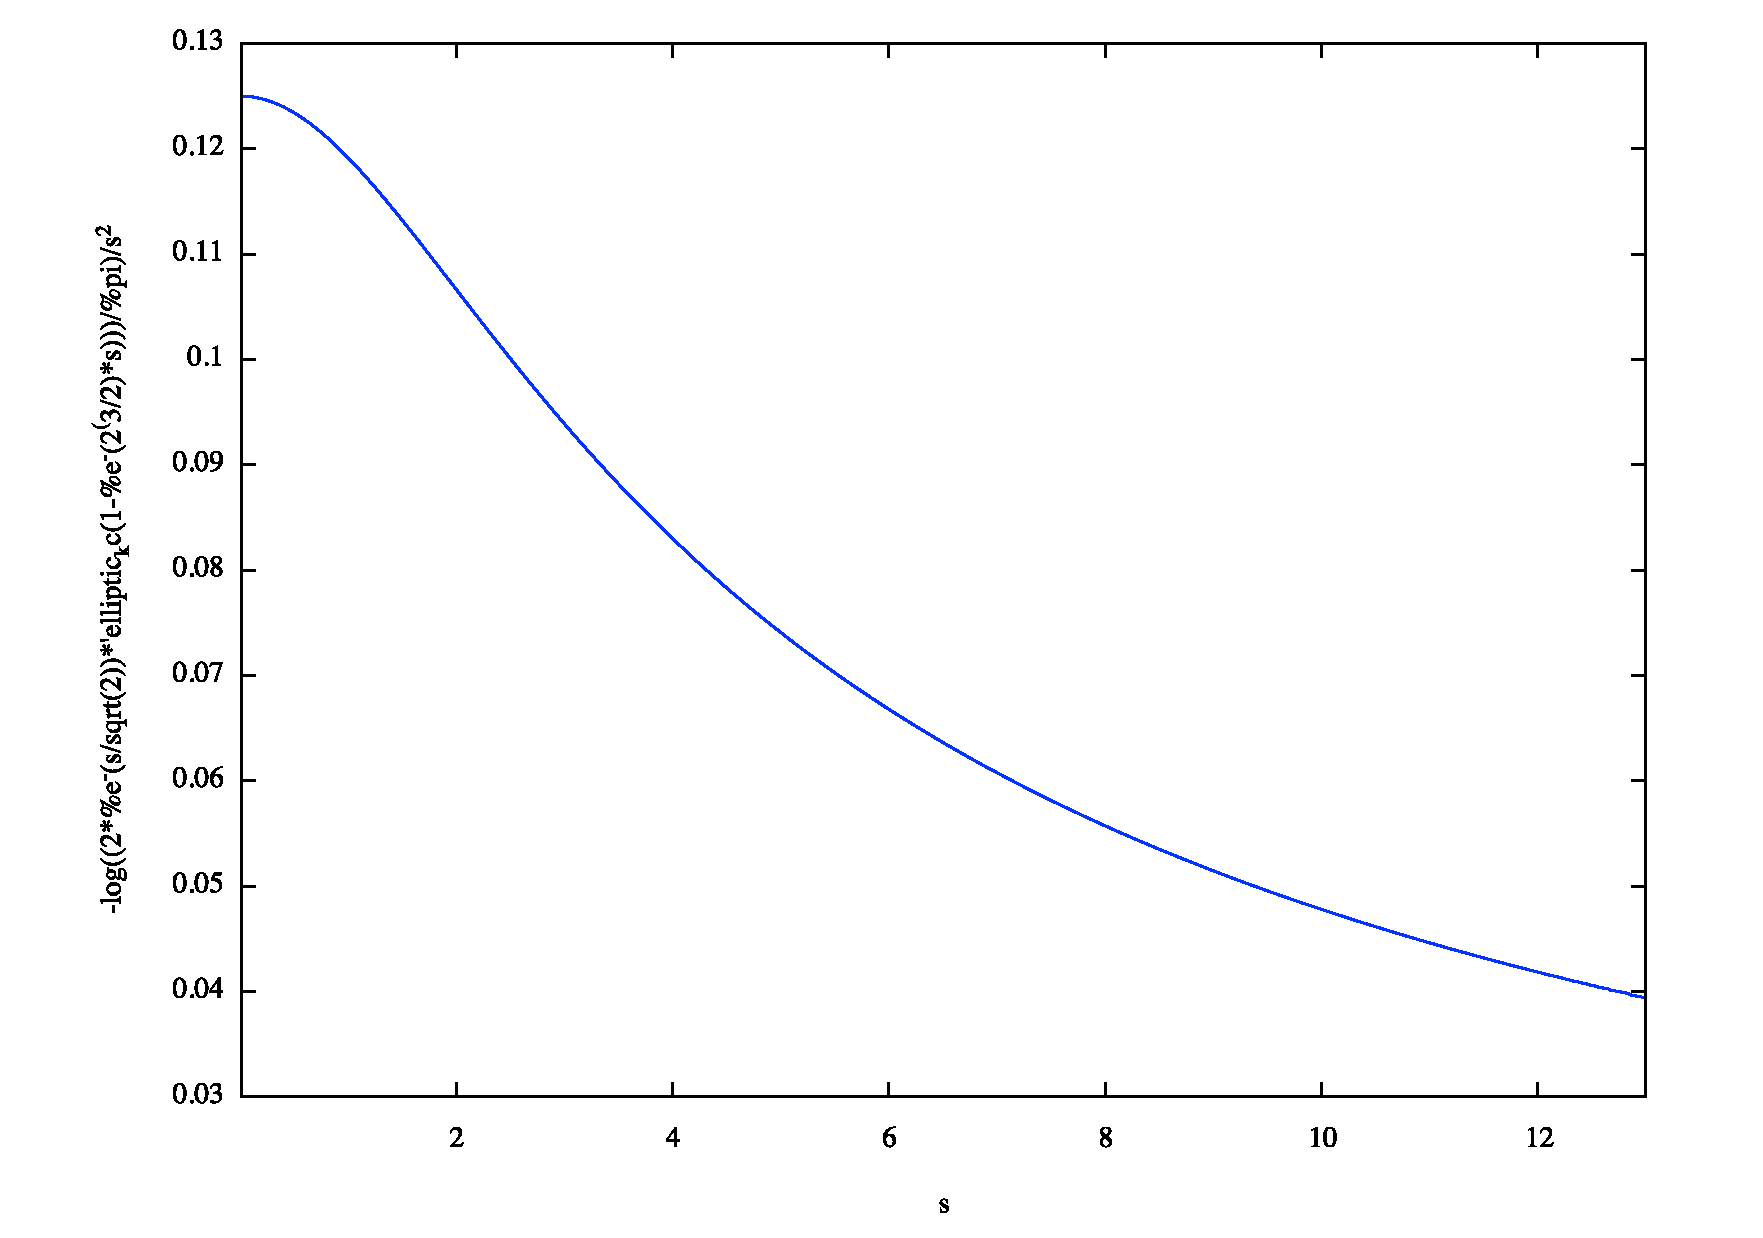
\includegraphics[width= 8cm, height= 6cm, bb= 0 0 846 594]{Figure-sqrt-Bhat-Cauchy.pdf}
\caption{Graph of $\frac{\sqrt{t_{\FR \rightarrow \Bhat}(s)}}{s}$}\label{fig:fig1}
\end{center}
\end{figure}




\subsection{Geometric properties of the metrizations of $f$-divergences}



If a divergence $D$ is given, then we can define an associated Riemannian metric $g_D$ on the parameter space by following Eguchi \cite{Eguchi1983, Eguchi1992}. 
Specifically, by regarding $D$ is a smooth function on $M \times M$ where $M$ is the space of parameters, 
we let 
\[ (g_D)_r (X_r, Y_r)  := -X_p Y_q\, D(p,q) |_{p=q=r}, \ r \in M, \]
where $X, Y$ are vector fields on $M$. 

It is known that if $D$ is the Kullback-Leibler divergence (or a standard $f$-divergence~\cite{IG-2016} with $f''(1)=1$), then, $g_D$ is the Fisher metric. 
If $D$ is not the Kullback-Leibler divergence, then, we are not sure whether $g_D$ is the Fisher metric. 
However, $g_D$ is the Fisher metric for every smooth $f$-divergence between the Cauchy distribution. 

\begin{proposition}\label{prop:local}
Let $I_f$ be the $f$-divergence between the location-scale family of the univariate Cauchy densities. 
Let $F$ be a function such that 
$$ I_f (p_{\theta_1} : p_{\theta_2}) = F(\chi(\theta_1, \theta_2)), \ \theta_1, \theta_2 \in \mathbb H.$$
Assume that $F$ is in $C^2 ([0, \infty))$. 
Then, the Riemannian metric $g_D$ is $F^{\prime}(0) \rho$, where $\rho$ is the Poincar\'e metric on $\mathbb H$. 
\end{proposition}


We remark that $\sqrt{2}\rho_{\textup{FR}}$ is identical with the Poincar\'e distance on $\mathbb H$.  



\begin{proposition}\label{prop:complete}
The square roots of the Kullback-Leibler and Bhattacharyya divergences between the location-scale family of the univariate Cauchy densities are both complete distances on $\mathbb H$. 
\end{proposition}

\begin{proof}
Assume that $(z_n)_n$ is a Cauchy sequence with respect to $ \sqrt{D_{\textup{KL}}}$. 
Since $\sqrt{D_{\textup{KL}}\left(p_{z} : p_{w}\right)}$ is increasing as a function of  $\chi(z,w)$, 
we see that 
$\chi(z_n, z_m) \to 0, n,m \to \infty$. 
We see that 
$\chi(z,w) \le \delta$ if and only if 
$$\left|w - (\textup{Re}(z) + i (1+\delta)\textup{Im}(z)) \right| \le \sqrt{\delta (\delta+2)} \textup{Im}(z). $$
Hence $(z_n)_n$ is bounded. 
Let $z$ be an accumulation point of $(z_n)_n$. 
Then, $z_{k_n} \to z, \ n \to \infty$ with respect to the Euclidean distance. 
Hence, 
$\chi(z_{k_n}, z) \to 0, n \to \infty$. 
Hence, 
$\sqrt{D_{\textup{KL}}\left(p_{z_{k_n}} : p_{z}\right)} \to 0, n \to \infty$. 
Since $(z_n)_n$ is a Cauchy sequence with respect to $ \sqrt{D_{\textup{KL}}}$, 
we see that 
$\sqrt{D_{\textup{KL}}\left(p_{z_{n}} : p_{z}\right)} \to 0, n \to \infty$. 
\end{proof}




We finally consider an isometric embedding of the kernel defined by the square root of the Kullback-Leibler divergence into a Hilbert space. 
The following is a significant extension of Theorem 4 in \cite{CauchyVoronoi-2020}. 

\begin{theorem}\label{thm:embeddable}
The square root of the Kullback-Leibler divergence between the location-scale family of the univariate Cauchy densities is isometrically embeddable into a Hilbert space. 
\end{theorem}

The method of the proof is completely different from the proof of Theorem 4 in \cite{CauchyVoronoi-2020}, 
because it cannot be a Bregman divergence. 
See also \cite{acharyya2013bregman}. 
Furthermore, Theorem 1 in \cite{fuglede2004jensen}, which gives a criteria whether a kernel is isometrically embeddable into a Hilbert space, will not be applicable to this setting.   
We give an elementary long proof of this assertion in Appendix \ref{sec:FH} in along with the following proof. 

\begin{proof}
By \cite{Schoenberg1938}, 
it suffices to show that $D_{\textup{KL}} (p_{z}:p_{w})$ is a conditionally negative definite kernel on $\mathbb H$, that is,  
for every $(c_1, \cdots, c_n)$ such that $\sum_{i=1}^{n} c_i = 0$ and every $z_1, \cdots, z_n \in \Theta$, 
\begin{equation}\label{eq:wts-ndk} 
\sum_{i,j=1}^{n} c_i c_j D_{\textup{KL}} (p_{z_i}:p_{z_j}) \le 0.
\end{equation}
We consider transformations of the parameter spaces from $\mathbb H$ to the hyperbolic plane in $\bbR^3$. 
Let 
\[ \mathbb L  := \{(x,y,z) \in \mathbb R^3 : z > 0, x^2 + y^2 - z^2 = -1\}. \]
Let 
\[ d_{\mathbb L} \left((x_1,y_1,z_1), (x_2,y_2,z_2)\right) \]
\[ := \cosh^{-1}\left( z_1 z_2 - x_1 x_2 - y_1 y_2 \right), (x_1,y_1,z_1), (x_2,y_2,z_2) \in \mathbb L.\]

Let $\phi_1 : \mathbb L \to \mathbb D$ be the map defined by $\phi_1(x,y,z) := \left(\frac{x}{1+z}, \frac{y}{1+z} \right)$.
 Let $\phi_2 : \mathbb D \to \mathbb H$ be the map defined by $\phi_2 (x,y) := \left(-\frac{2y}{(1-x)^2 + y^2}, \frac{1-x^2-y^2}{(1-x)^2 + y^2}\right)$.
Then, $\phi_1$ and $\phi_2$ are both bijective. 
Hence $\phi_2 \circ \phi_1$ is a bijection between $\mathbb H$ and $\mathbb L$. 

Hence, in order to show \eqref{eq:wts-ndk}, 
it suffices to show that for $(x_1, y_1, z_1), \cdots, (x_n, y_n, z_n) \in \mathbb L$, 
\[ \sum_{i,j=1}^{n} c_i c_j \log\left(1+ \frac{\chi\left(\phi_2 (\phi_1(x_i,y_i,z_i)), \phi_2 (\phi_1(x_j,y_j,z_j))\right)}{2}\right) \le 0. \]

Since
\[ \chi(\phi_2 (w_1), \phi_2 (w_2)) = \frac{2|w_1 - w_2|^2}{(1-|w_1|^2)(1-|w_2|^2)}, \ \ w_1, w_2 \in \mathbb D, \]
we see that for $(x_1,y_1,z_1), (x_2,y_2,z_2) \in \mathbb L$, 
\[ \chi\left(\phi_2 (\phi_1(x_1,y_1,z_1)), \phi_2 (\phi_1(x_2,y_2,z_2))\right) \]
\[ = 
\cosh\left(d_{\mathbb L}\left((x_1,y_1,z_1), (x_2,y_2,z_2)\right)\right)-1. \]

Hence, in order to show \eqref{eq:wts-ndk}, 
it suffices to show that for $(x_1, y_1, z_1), \cdots, (x_n, y_n, z_n) \in \mathbb L$, 
\[ \sum_{i,j=1}^{n} c_i c_j \log\left(\frac{1+\cosh\left(d_{\mathbb L}\left((x_i,y_i,z_i), (x_j,y_j,z_j)\right)\right)}{2}\right) \le 0. \]
Since $2(\cosh (x/2))^2 = 1 + \cosh(x), x \in \mathbb R$, 
in order to show \eqref{eq:wts-ndk}, 
it suffices to show that for $(x_1, y_1, z_1), \cdots, (x_n, y_n, z_n) \in \mathbb L$, 
\begin{equation}\label{eq:wts-FH} 
\sum_{i,j=1}^{n} c_i c_j 2\log\left( \cosh \left(\frac{d_{\mathbb L}\left((x_i,y_i,z_i), (x_j,y_j,z_j)\right)}{2}\right) \right) \le 0. 
\end{equation}

The last inequality follows from Theorem 7.5 in Faraut-Harzallah \cite{Faraut-1974}. 
\begin{theorem}[Theorem 7.5 in Faraut-Harzallah \cite{Faraut-1974}]
Let $d \ge 2$. 
For $x = (x_1, \cdots, x_d) \in \bbR^d$ and $y = (y_1, \cdots, y_d) \in \bbR^d$,
let 
\[ r(x,y) := \]
\[ \cosh^{-1} \left(\sqrt{\left(1+\sum_{i=1}^{d} x_i^2\right)\left(1+\sum_{i=1}^{d} y_i^2\right)} - \sum_{i=1}^{d} x_i y_i\right) \]
and 
\[ Q(x,y) := \frac{\Gamma(\frac{d}{2})}{\sqrt{\pi} \Gamma(\frac{d-1}{2})} \times\]
\[ \int_0^{\pi} \log\left( \cosh(r(x,y)) - \cos\theta \sinh(r(x,y)) \right) \sin^{d-2} \theta d\theta. \]
Then, $Q$ is a conditionally negative definite kernel on $\mathbb{R}^d$, specifically, 
for every $(c_1, \cdots, c_n)$ such that $\sum_{i=1}^{n} c_i = 0$ and every $z_1, \cdots, z_n \in \bbR^d$, 
\begin{equation*}
\sum_{i,j=1}^{n} c_i c_j Q(z_i, z_j) \le 0.
\end{equation*}
\end{theorem}

We apply this theorem to the case that $d=2$. 
Then, we see that for $x = (x_1, x_2)$ and $y = (y_1, y_2)$,
\[ r(x,y) \]
\[= d_{\mathbb L}\left(\left(x_1, x_2, \sqrt{1+x_1^2+x_2^2}\right), \left(y_1, y_2, \sqrt{1+y_1^2+y_2^2}\right)\right), \]
and 
\[ Q(x,y) = \frac{1}{\pi} \int_0^{\pi} \log\left( \cosh(r(x,y)) - \cos\theta \sinh(r(x,y)) \right) d\theta. \]
The formula no.4.224.9 in \cite{gradshteyn2014table} states that 
\[ 2 \log \cosh \left(\frac{r}{2}\right) = \frac{1}{2\pi} \int_{-\pi}^{\pi} \log\left(\cosh(r) + \cos\theta \sinh (r) \right) d\theta \]
\[= \frac{1}{\pi} \int_{0}^{\pi} \log\left(\cosh(r) + \cos\theta \sinh (r) \right) d\theta,  r \ge 0. \]
Hence, 
\[ Q(x,y) = 2 \log \cosh \left(\frac{r(x,y)}{2}\right). \]
Thus \eqref{eq:wts-FH} holds. 
\end{proof}


\begin{remark}\label{rem:FH}
(i) 
Faraut-Harzallah \cite{Faraut-1974} often uses terminologies of representation theory. 
The proof of Theorem 7.5 in Faraut-Harzallah \cite{Faraut-1974} heavily depends on Takahashi's long paper \cite{Takahashi-1963} in representation theory.  
Another paper of Faraut-Harzallah \cite{Faraut-1972} gave another derivation of  Theorem 7.5 in \cite{Faraut-1974}. 
However, \cite{Faraut-1972} heavily depends on Helgason's long paper \cite{Helgason-1970} in representation theory.  
By following the outline of \cite{Faraut-1972}, 
we give an elementary, long proof of Theorem \ref{thm:embeddable}  in Appendix \ref{sec:FH} without using any terminologies of representation theory.  \\
(ii) Theorem 8.1 in \cite{Faraut-1974} proved some results on positive and negative definite kernels defined on a real infinite dimensional hyperbolic space. 
It is similar to Theorem 7.5 in \cite{Faraut-1974}, but is different and we cannot apply the result to our case.  
See  Chapter5, Section 5 in Berg, Christensen and Ressel \cite{Berg1984} for details. 
\cite{Faraut-1974} gives some interesting examples of conditionally negative definite kernels on Euclidian spaces of every dimension. 
\end{remark}


\begin{remark}
We can show that neither $(\mathbb H, \sqrt{D_{\textup{Bhat}}})$ nor $(\mathbb H, \sqrt{D_{\textup{KL}}})$ is a geodesic metric space. 
Now by Hopf-Rinow's theorem (see \cite[Theorem 16]{Petersen2006}) and Proposition  \ref{prop:complete}, 
neither $\sqrt{D_{\textup{Bhat}}}$ or $\sqrt{D_{\textup{KL}}}$ is a Riemannian distance. 
Furthermore, we can also show that neither $(\mathbb H, \sqrt{D_{\textup{Bhat}}})$ nor $(\mathbb H, \sqrt{D_{\textup{KL}}})$ is Gromov-hyperbolic. 
Now we see that both of the metrics  $\sqrt{D_{\textup{Bhat}}}$ and $\sqrt{D_{\textup{KL}}}$ are locally similar to the Poincar\'e metric (recall Proposition \ref{prop:local}), however, in global, they are completely different from the Poincar\'e metric.
See \cite{Nielsen2021f} for details. 
\end{remark}


%\subsection{Subsection Heading Here}
%Subsection text here.

% needed in second column of first page if using \IEEEpubid
%\IEEEpubidadjcol

%\subsubsection{Subsubsection Heading Here}
%Subsubsection text here.


% An example of a floating figure using the graphicx package.
% Note that \label must occur AFTER (or within) \caption.
% For figures, \caption should occur after the \includegraphics.
% Note that IEEEtran v1.7 and later has special internal code that
% is designed to preserve the operation of \label within \caption
% even when the captionsoff option is in effect. However, because
% of issues like this, it may be the safest practice to put all your
% \label just after \caption rather than within \caption{}.
%
% Reminder: the "draftcls" or "draftclsnofoot", not "draft", class
% option should be used if it is desired that the figures are to be
% displayed while in draft mode.
%
%\begin{figure}[!t]
%\centering
%\includegraphics[width=2.5in]{myfigure}
% where an .eps filename suffix will be assumed under latex, 
% and a .pdf suffix will be assumed for pdflatex; or what has been declared
% via \DeclareGraphicsExtensions.
%\caption{Simulation results for the network.}
%\label{fig_sim}
%\end{figure}

% Note that the IEEE typically puts floats only at the top, even when this
% results in a large percentage of a column being occupied by floats.


% An example of a double column floating figure using two subfigures.
% (The subfig.sty package must be loaded for this to work.)
% The subfigure \label commands are set within each subfloat command,
% and the \label for the overall figure must come after \caption.
% \hfil is used as a separator to get equal spacing.
% Watch out that the combined width of all the subfigures on a 
% line do not exceed the text width or a line break will occur.
%
%\begin{figure*}[!t]
%\centering
%\subfloat[Case I]{\includegraphics[width=2.5in]{box}%
%\label{fig_first_case}}
%\hfil
%\subfloat[Case II]{\includegraphics[width=2.5in]{box}%
%\label{fig_second_case}}
%\caption{Simulation results for the network.}
%\label{fig_sim}
%\end{figure*}
%
% Note that often IEEE papers with subfigures do not employ subfigure
% captions (using the optional argument to \subfloat[]), but instead will
% reference/describe all of them (a), (b), etc., within the main caption.
% Be aware that for subfig.sty to generate the (a), (b), etc., subfigure
% labels, the optional argument to \subfloat must be present. If a
% subcaption is not desired, just leave its contents blank,
% e.g., \subfloat[].


% An example of a floating table. Note that, for IEEE style tables, the
% \caption command should come BEFORE the table and, given that table
% captions serve much like titles, are usually capitalized except for words
% such as a, an, and, as, at, but, by, for, in, nor, of, on, or, the, to
% and up, which are usually not capitalized unless they are the first or
% last word of the caption. Table text will default to \footnotesize as
% the IEEE normally uses this smaller font for tables.
% The \label must come after \caption as always.
%
%\begin{table}[!t]
%% increase table row spacing, adjust to taste
%\renewcommand{\arraystretch}{1.3}
% if using array.sty, it might be a good idea to tweak the value of
% \extrarowheight as needed to properly center the text within the cells
%\caption{An Example of a Table}
%\label{table_example}
%\centering
%% Some packages, such as MDW tools, offer better commands for making tables
%% than the plain LaTeX2e tabular which is used here.
%\begin{tabular}{|c||c|}
%\hline
%One & Two\\
%\hline
%Three & Four\\
%\hline
%\end{tabular}
%\end{table}


% Note that the IEEE does not put floats in the very first column
% - or typically anywhere on the first page for that matter. Also,
% in-text middle ("here") positioning is typically not used, but it
% is allowed and encouraged for Computer Society conferences (but
% not Computer Society journals). Most IEEE journals/conferences use
% top floats exclusively. 
% Note that, LaTeX2e, unlike IEEE journals/conferences, places
% footnotes above bottom floats. This can be corrected via the
% \fnbelowfloat command of the stfloats package.




\section{Conclusion and Discussion}\label{sec:concl}
%%%
 
In this work, we first proved that all $f$-divergences~\cite{csiszar2004information} between univariate Cauchy distributions are symmetric by handling the parameters of Cauchy distributions as complex numbers and considering the action of the M\"obius group~\cite{mccullagh1996mobius}.  
We showed that those $f$-divergences can be calculated as strictly increasing scalar functions of the chi-square divergence by using the notion of maximal invariant~\cite{Eaton-1989,mccullagh1992conditional}. 
However, we showed that the $f$-divergences between multivariate Cauchy densities are in general asymmetric by reporting an example, 
but on the other hand, proved that $f$-divergences between multivariate Cauchy divergences are symmetric when the Cauchy scale matrices coincide. 
We also reported a criterion for expanding $f$-divergences as converging series of power chi divergences, and illustrated the technique for some common $f$-divergences between Cauchy distributions. 
Finally, we proved that the square roots of the Kullback-Leibler and the Bhattacharyya divergences between univariate Cauchy distributions yield both complete metric spaces, and the square root of the Kullback-Leibler divergence between univariate Cauchy distributions is isometrically embeddable into a Hilbert space. 

When divergences are symmetric, the induced divergence-based information $\alpha$-geometry~\cite{IG-2016} all coincide with the Fisher-Rao geometry (i.e., the $0$-geometry)
 (equivalently, the Amari-Chentsov symmetric cubic tensor vanishes).
When parametric families belong to exponential families, the only families which yield symmetric KL divergences are provably location normal distributions.
Indeed, the KLD between two densities of an exponential family amounts to an equivalent Bregman divergence and the only symmetric Bregman divergences
are squared Mahalanobis divergences~\cite{BVD-2010}.
In this paper, we proved that all $f$-divergences between Cauchy densities are symmetric.
Once such a family is found, we may consider diffeomorphisms $y=m(x)$ which keeps the $f$-divergences invariant
but yield other parametric families of distributions (e.g., circular, wrapped, or log-Cauchy families).
Notice that the Cauchy densities  are infinitely divisible distributions and can thus be realized as scale mixtures of Gaussian density functions
(see \url{https://betanalpha.github.io/assets/case_studies/fitting_the_cauchy.html}).

To conclude, let us state an interesting open problem raised by our work:
\begin{problem}
Characterize all parametric distribution families $\{p_\theta\}_\theta$ (and transformational models ~\cite{StatTransfModel-2012}) for which the Kullback-Leibler divergence
 (or more generally any $f$-divergence) is symmetric.
\end{problem}







% if have a single appendix:
%\appendix[Proof of the Zonklar Equations]
% or
%\appendix  % for no appendix heading
% do not use \section anymore after \appendix, only \section*
% is possibly needed

% use appendices with more than one appendix
% then use \section to start each appendix
% you must declare a \section before using any
% \subsection or using \label (\appendices by itself
% starts a section numbered zero.)
%


\appendices
%\section{Proof of ????}
%Appendix one text goes here.

\section{Complete elliptic integrals}\label{sec:cei}
%%%

This section is devoted to the details of the proof of \eqref{eq:sqrt-Bhat} in the proof of Theorem \ref{thm:sqrtBhat}. 
Let $\mathbf{E}$ be the complete elliptic integral of the second kind. 
We let\footnote{This is also a little different from the usual definition. The usual one is $\mathbf{E}(t) = \int_0^{\pi/2} \sqrt{1 - t^2 \sin^2 \theta} d\theta.$} 
\[ \mathbf{E}(t) := \int_0^{\pi/2} \sqrt{1 - t \sin^2 \theta} d\theta. \]

\begin{proof}
Let
\[ F_4(u) := \frac{-\log\left(2 e^{-u/4} \mathbf{K}(1-e^{-u}) /\pi \right)}{u^2}. \]

We consider the derivative. 
\[ F_4^{\prime}(u) = \]
\[\frac{-1}{u^2} \left( \frac{1}{4} + e^{-u} \frac{\mathbf{K}^{\prime}(1-e^{-u})}{\mathbf{K}(1-e^{-u})} - \frac{2}{u} \log\left(\frac{2}{\pi}\mathbf{K}(1-e^{-u}) \right) \right). \]

Now it suffices to show that for every $u > 0$, 
\[ \frac{1}{4} + e^{-u} \frac{\mathbf{K}^{\prime}(1-e^{-u})}{\mathbf{K}(1-e^{-u})} - \frac{2}{u} \log\left(\frac{2}{\pi}\mathbf{K}(1-e^{-u}) \right) > 0. \] 

Let $x := 1 - e^{-u}$. 
Then, it suffices to show that for every $x \in (0,1)$, 
\[  \frac{1}{4} + (1-x) \frac{\mathbf{K}^{\prime}(x)}{\mathbf{K}(x)} + \frac{2}{\log(1-x)} \log\left(\frac{2}{\pi} \mathbf{K}(x) \right) > 0. \]
Let 
\[ G_4(x) := \log\left(\frac{2}{\pi} \mathbf{K}(x) \right) + (\log(1-x))\left( \frac{1}{8} + \frac{1-x}{2} \frac{\mathbf{K}^{\prime}(x)}{\mathbf{K}(x)}  \right). \]
It suffices to show that $G_4(x) < 0$ for every $x \in (0,1)$. 

We see that $G(0) = 0$. 
Hence it suffices to show that $G^{\prime}(x) < 0$ for every $x \in (0,1)$. 
By Lemma \ref{K-deri} below, 
\[ G_4(x) = \]  
\[\log\left(\frac{2}{\pi} \mathbf{K}(x) \right) + (\log(1-x))\left( \frac{3}{8} + \frac{1}{4x} \left( \frac{\mathbf{E}(x)}{\mathbf{K}(x)} - 1\right) \right). \]

By Lemmas \ref{K-deri} and \ref{EK-deri} below, 
\[ G_4^{\prime}(x) = -\frac{H_4(x)}{8x^2 (1-x)}, \]
where we let 
\[ H_4(x) := (x(2-x) + (x-1)\log(1-x)) \mathbf{K}(x)^2 \] 
\[ -2x \mathbf{K}(x)\mathbf{E}(x) + \log(1-x) \mathbf{E}(x)^2. \]
Then it suffices to show that $H_4(x) > 0$ for every $x \in (0,1)$. 
Since $-2x < 0$ and $ \log(1-x) < 0$, 
by noting Lemma \ref{Gauss-AGM} below, 
it holds that 
\[ \frac{\mathbf{H}(x)}{\mathbf{K}(x)^2} \ge  (x(2-x) + (x-1)\log(1-x))\]
\[ -2x I_4(x) + \log(1-x) I_4(x)^2, \]
where we let 
\[ I_4(x) := \frac{1}{2} - \frac{x}{4} + \frac{\sqrt{1-x}}{2}. \]

Our main idea is to use different estimates for $H(x)/\mathbf{K}(x)^2$ on a neighborhood of $1$ and on the complement of it. 

\begin{lemma}
For $x \le 0.998$, 
\[ (x(2-x) + (x-1)\log(1-x)) > 2x I_4(x) + \log(1-x) I_4(x)^2.\]
\end{lemma}

\begin{proof}
Let $y := \sqrt{1-x}$. 
Then, 
\[ (x(2-x) + (x-1)\log(1-x)) > 2x I(x) + \log(1-x) I(x)^2 \]
is equivalent with 
\[ \log y > 4\frac{y^2 -1}{y^2 + 6y + 1}. \]
Let $$P_4 (y) := \log y - 4\frac{y^2 -1}{y^2 + 6y + 1}.$$ 
Then, $P_4 (1) = 0$. 
By considering the derivative of $P_4 $, 
it is increasing $y < 5 - 2\sqrt{6}$ and decreasing $y > 5 - 2\sqrt{6}$. 

We see that 
$
P_4 (y) > 0 \ \ y > 0.041.
$
Now the assertion follows from the fact that 
$0.998 < 1 - (0.041)^{2}$.
\end{proof}

Now it suffices to show that $H_4 (x) > 0$ for $x > 0.998$. 


\begin{lemma}\label{lem:1st}
\[ x(2-x) + (x-1)\log(1-x) \ge 1, \ \ x \in (0.998,1). \]
\end{lemma}

\begin{proof}
Let $g_4(x) := x(2-x) + (x-1)\log(1-x)$. 
Then, $g(1) = 1$ and 
$g_4^{\prime}(x) = 3-2x + \log(1-x)$. 
This is negative if $x > 0.9$. 
\end{proof}

\begin{lemma}\label{lem:2nd}
\[ 2x \frac{\mathbf{E}(x)}{\mathbf{K}(x)} < \frac{1}{2}, \ \ x \in (0.998,1). \]
\end{lemma}

\begin{proof}
We see that 
\[ \frac{d}{dx} \left( x \frac{\mathbf{E}(x)}{\mathbf{K}(x)}\right) \le  2\frac{\mathbf{E}(x)}{\mathbf{K}(x)}  -\frac{1}{2}. \]

By Lemma \ref{EK-deri}  below and the fact that 
\[ \frac{\mathbf{E}(0.995)}{\mathbf{K}(0.995)} < \frac{1}{4},\] 
we see that 
\[  2\frac{\mathbf{E}(x)}{\mathbf{K}(x)}  \le \frac{1}{2}, \ \ x > 0.995. \]

Hence, 
\[ 2x \frac{\mathbf{E}(x)}{\mathbf{K}(x)} < 2 \frac{\mathbf{E}(0.995)}{\mathbf{K}(0.995)} < \frac{1}{2}. \]
\end{proof}


\begin{lemma}\label{lem:3rd}
\[ -\log(1-x) \left( \frac{\mathbf{E}(x)}{\mathbf{K}(x)}  \right)^2 < \frac{1}{2},  x \in (0.998,1). \]
\end{lemma}


\begin{proof}
We use Lemma \ref{AVV} below. 
It suffices to show that 
\[  \frac{2 x^{1/2}}{\log(1+x^{1/2}) - \log(1-x^{1/2})} \le \sqrt{\frac{1}{-2\log(1-x)}}  \]
for $x \in (0.998,1)$. 
This is equivalent with 
\[ h_4(x) := \left( \log(1+x^{1/2}) - \log(1-x^{1/2}) \right)^2 + 8x\log(1-x) \ge 0   \]
for $x \in (0.998,1)$. 
We see that 
\[ -\frac{h_4^{\prime}(x)}{2} = \]
\[\frac{\log(1-\sqrt{x}) - \log(1+\sqrt{x}) + 2\sqrt{x}(x + (x-1)\log(1-x))}{(1-x)\sqrt{x}}. \]

It is easy to see that 
\[ \log(1-\sqrt{x}) - \log(1+\sqrt{x}) + 2\sqrt{x}(x + (x-1)\log(1-x)) < 0  \]
for $x \in (0.998,1)$.
Hence $h_4$ is increasing at least on $(0.998,1)$.  
Now use the fact that $h_4(0.998) > 0$. 
\end{proof}



By Lemmas \ref{lem:1st}, \ref{lem:2nd} and \ref{lem:3rd}, 
we see that $H_4(x) > 0$ for $x > 0.998$. 
The proof of \eqref{eq:sqrt-Bhat} is completed. 
\end{proof}

\subsubsection{Some Lemmas concerning the complete elliptic integrals}

We collect standard results about the complete elliptic integrals. 

\begin{lemma}\label{K-deri}
\[ \mathbf{K}^{\prime}(x) = -\frac{\mathbf{K}(x)}{2x} + \frac{\mathbf{E}(x)}{2x(1-x)}. \]
\end{lemma}

\begin{lemma}\label{EK-deri}
\[ \frac{d}{dx}\left(\frac{\mathbf{E}(x)}{\mathbf{K}(x)} \right) = -\frac{1}{2x} + \frac{1}{x} \frac{\mathbf{E}(x)}{\mathbf{K}(x)} - \frac{1}{2x(1-x)} \left( \frac{\mathbf{E}(x)}{\mathbf{K}(x)}\right)^2 \le 0. \]
In particular, 
$\mathbf{E}/\mathbf{K}$ is strictly decreasing. 
\end{lemma}

\begin{lemma}\label{Gauss-AGM}
\[ \frac{\mathbf{E}(x)}{\mathbf{K}(x)} \le \frac{1}{2} - \frac{x}{4} + \frac{\sqrt{1-x}}{2}, \ x \in [0,1).\]
\end{lemma}

The following is due to Anderson,  Vamanamurthy, and Vuorinen \cite{AVV}. 

\begin{lemma}[{\cite[Theorem 3.6]{AVV}}]\label{AVV}
\[  \frac{\mathbf{E}(x)}{\mathbf{K}(x)} \le \frac{2 x^{1/2}}{\log(1+x^{1/2}) - \log(1-x^{1/2})}, \ x \in [0,1). \]
\end{lemma}

%%%
\section{Negative definiteness of the KLD between Cauchy densities}\label{sec:FH}
%%%

In this section, we give an elementary but long proof of Theorem \ref{thm:embeddable}. 
We first give an outline of the alternative proof. 
Our proof follows the strategy of \cite{Faraut-1972} and consists of three steps. 
Contrarily to the proof of  Theorem \ref{thm:embeddable} given in Section \ref{sec:metrization},  
we do not need to introduce the hyperboloid space $\mathbb L$. 


\begin{proof}[Outline of Proof of Theorem \ref{thm:embeddable}]
By \cite{Schoenberg1938}, 
it suffices to show that $D_{\textup{KL}} (p_{z}:p_{w})$ is a conditionally negative definite kernel on $\mathbb H$, that is,  
for every $(c_1, \cdots, c_n)$ such that $\sum_{i=1}^{n} c_i = 0$ and every $z_1, \cdots, z_n \in \Theta$, 
\begin{equation*}
\sum_{i,j=1}^{n} c_i c_j D_{\textup{KL}} (p_{z_i}:p_{z_j}) 
= \sum_{i,j=1}^{n} c_i c_j  \log \left( 1 + \frac{\chi(z_i,z_j)}{2} \right) \le 0.
\end{equation*}

If we find a positive-definite kernel $H_s$ on $\mathbb H$ for each $s > 0$ such that 
\[ \log \left( 1 + \frac{\chi(z,w)}{2} \right) = \lim_{s \to +0} \frac{1-H_s (z,w)}{s}, \ \ z, w \in \mathbb H, \]
then, for each $s > 0$, 
$1-H_s (z,w)$ is a conditionally negative definite kernel on $\mathbb H$ and hence $\log \left( 1 + \frac{\chi(z,w)}{2} \right)$ is also 
a conditionally negative definite kernel on $\mathbb H$. 

Step 1. \ Let $d$ be the Poincar\'e distance on $\mathbb H$, which is equal to $\sqrt{2}\rho_{\textup{FR}}$. 
Then, $\cosh(d(z,w)) = 1 + \chi(z,w)$ and  
$$2 \log \cosh \left(\frac{d(z,w)}{2} \right) = \log \left( 1 + \frac{\chi(z,w)}{2} \right).$$  

We see that for every $r \ge 0$, 
\[ 2 \log \cosh \left(\frac{r}{2} \right) \]
\[= \lim_{s \to +0} \frac{1}{s} \left( 1 - \frac{1}{2\pi} \int_{-\pi}^{\pi}  \left( \cosh(r) + \cos \theta \sinh (r) \right)^{-s} d\theta \right).\]

Hence it suffices to show that 
\[ H_s (z,w) := \]
\[\frac{1}{2\pi} \int_{-\pi}^{\pi}  \left( \cosh(d(z,w)) + \cos \theta \sinh (d(z,w)) \right)^{-s} d\theta, z,w \in \mathbb H, \]
is positive definite for every $s \in (0,1)$. \\

Step 2. \ Let 
\[ P(z,x) := \frac{\textup{Im}(z)}{|x-z|^2} (x^2 + 1), \ z \in \mathbb H, x \in \mathbb R, \]
and,  
\[ \mu(dx) := \dfrac{dx}{\pi (x^2 + 1)}, \ x \in \mathbb{R}.\]

Then we see that 
\[ H_s (z,w) = \int_{\mathbb R} P(z,x)^s P(w,x)^{1-s} \mu(dx) = \]
\[ C_s \int_{\mathbb R^2} (P(w,x)P(z,y))^{1-s} \left( \frac{(x-y)^2}{(x^2 + 1) (y^2 + 1)} \right)^{-s} \mu(dx)\mu(dy), \]
where $C_s$ is a positive constant depending only on $s$. \\

Step 3. \ Let $z_1, \cdots, z_n \in \mathbb H$ and $c_1, \cdots, c_n \in \mathbb R$ with $\sum_{i=1}^{n} c_i = 0$. 
Let 
\begin{equation}\label{def-varphi_s}
\varphi_s (x) := \sum_{i=1}^{n} c_i P(z_i, x)^{1-s}, \ x \in \mathbb R,
\end{equation} 
which is continuous on $\mathbb R$.  
Let 
\begin{equation}\label{def-k_s}
k_s (x,y) := \left( \frac{(x-y)^2}{(x^2 + 1) (y^2 + 1)} \right)^{-s}, 
\end{equation} 
which is a positive definite kernel on $\mathbb R$. 

Thus we see that 
\[ \sum_{i.j=1}^{n} c_i c_j H_s (z_i, z_j) = \frac{C_s}{\pi^2} \iint_{\mathbb R^2} \frac{\varphi_s (x) \varphi_s (y) k_s (x,y)}{(x^2 + 1)(y^2 + 1)} dxdy \ge 0. \]
In order to show the last inequality, we use a certain approximation for $k_s$.  
\end{proof}
 
Now we proceed to the full proof. 

\begin{proof}[Proof of Theorem \ref{thm:embeddable}]
Step 1. \ 
It is known that (see formula no.4.224.9 in \cite{gradshteyn2014table})
\[ 2 \log \cosh \left(\frac{r}{2}\right) \]
\[= \frac{1}{2\pi} \int_{-\pi}^{\pi} \log\left(\cosh(r) + \cos\theta \sinh (r) \right) d\theta,  \ r \ge 0. \]

We see that for $r \ge 0$, 
\[ \left|\log (\cosh(r) + \cos\theta \sinh (r)) \right| \le r.  \]

Since for $t > 0$, $\displaystyle\lim_{s \to +0} \frac{1 - t^{-s}}{s} = \log t$ 
and $\displaystyle\left|\frac{1 - t^{-s}}{s}\right| \le |\log t|$, 
\[ \int_{-\pi}^{\pi} \log\left(\cosh(r) +\cos\theta \sinh(r) \right) d\theta \]
\[= \lim_{s \to +0} \int_{-\pi}^{\pi} \frac{1 - \left(\cosh(r) +\cos\theta \sinh (r) \right)^{-s}}{s}d\theta, r > 0, \]
by the Lebesgue convergence theorem. 
This convergence also holds for $r=0$. 
This completes Step 1. \\  

Step 2. \ This part is the longest.  
\begin{lemma}\label{lem:transfer}
\[ \frac{1}{2\pi} \int_{-\pi}^{\pi} \left(\cosh(r) +\cos\theta \sinh (r) \right)^{-s} d\theta = \int_{\mathbb R} P(e^r i, x)^s \mu(dx).  \]
\end{lemma}

\begin{proof}
Let $x = \tan \frac{\theta}{2}$. 
Then, 
$d\theta = \dfrac{2}{1+x^2} dx$ and 
\[ \cosh(r) +\cos\theta \sinh (r) = \frac{e^{2r} + x^2}{e^r (1+x^2)} = \frac{1}{P(e^r i, x)}. \]
\end{proof}

\begin{lemma}\label{lem:rot-inv}
For $A \in \mathrm{SO}(2)$ and $z \in \mathbb H$, 
\[ \int_{\mathbb R} P(A.z,x)^s \mu(dx) =  \int_{\mathbb R} P(z,x)^s \mu(dx). \]
\end{lemma}

\begin{proof}
Let 
$A = \begin{pmatrix} \cos\theta & -\sin\theta \\ \sin\theta & \cos\theta \end{pmatrix}$. 
Let $y \in \mathbb R$ such that $x = A.y$. 
Then, $P(A.z, A.y) = P(z,y)$ 
and 
\[ \mu(dx) = \frac{1}{\pi} \frac{1}{(A.y)^2 + 1} \frac{dx}{dy} dy = \frac{1}{\pi} \frac{1}{y^2 + 1} dy = \mu(dy). \]
\end{proof}

Now we introduce a group structure on $\mathbb H$. 
For $z = z_1+iz_2$ and $w = w_1+iw_2$, let $zw := (z_1 + z_2 w_1) + i z_2 w_2$.
This gives a group structure on $\mathbb H$. 
It holds that 
$$ w^{-1} = \frac{-w_1 + i}{w_2}, \ w = w_1+iw_2$$
and the unit element is the imaginary unit $i$. 

We see that 
$\chi(w^{-1}z,i) = \chi(z,w), z,w \in \mathbb H$ and hence 
\begin{equation}\label{eq:gi-dist}
d(w^{-1}z,i) = d(z,w), z,w \in \mathbb H.
\end{equation} 



\begin{lemma}\label{lem:inverse}
For $z,w \in \mathbb H$, 
\[ H_s (z,w) = \int_{\mathbb R} P(w^{-1} z, x)^s \mu(dx).  \]
\end{lemma}


\begin{proof}
By \eqref{eq:gi-dist}, we can assume that $w=i$. 
Then there exists $A \in SO(2)$ such that $e^{d(z,i)} i = A.z$. 
Now the assertion follows from Lemmas \ref{lem:transfer} and \ref{lem:rot-inv}. 
\end{proof}

For $w = w_1 + iw_2 \in \mathbb H$ and $x \in \mathbb R$, 
we let $wx := w_2 x + w_1$.

\begin{lemma}\label{lem:ratio}
\[ P(w^{-1}z, x) P(w, wx) = P(z, wx), \ \ z, w \in \mathbb H, x \in \mathbb R. \]
\end{lemma}

\begin{proof}
Since 
\[ w^{-1}z = \frac{z_1 - w_1 + i z_2}{w_2}, \ \ z = z_1 + iz_2, w = w_1 + iw_2, \]
we see that 
\[ P(w^{-1}z, x) = \frac{z_2 w_2}{(z_1 - w_1 - w_2 x)^2 + z_2^2} (x^2 + 1). \]
We also see that 
\[ P(z,wx) = \frac{z_2 ((w_2 x + w_1)^2+1)}{(z_1 - w_1 - w_2 x)^2 + z_2^2} \] 
and \[ P(w,wx) = \frac{(w_2 x + w_1)^2+1}{w_2 (x^2 + 1)}. \]
The assertion follows from these identities. 
\end{proof}

\begin{proposition}\label{prop:prop1}
\[ H_s (z,w) = \int_{\mathbb R} P(z,x)^s P(w,x)^{1-s} \mu(dx), \ \ z, w \in \mathbb H.\] 
\end{proposition}

\begin{proof}
By Lemmas \ref{lem:inverse} and \ref{lem:ratio}, 
\[ H_s (z,w) = \int_{\mathbb R} P(z, wx)^s P(w, wx)^{-s} \mu(dx). \]
Let $y = wx = w_2 x + w_1$. 
Then, $\mu(dx) = \dfrac{w_2}{\pi |y-w|^2} dy$. 
Hence, 
\[ \int_{\mathbb R} P(z, wx)^s P(w, wx)^{-s} \mu(dx) = \int_{\mathbb R} P(z,y)^s P(w,y)^{1-s} \mu(dy). \]
\end{proof}

\begin{lemma}\label{lem:intertwin-pre}
For every $s \in (0,1/2)$, there exists a positive constant $C_s$ such that for every $a \in \mathbb R$ 
\[ (1+a^2)^{-s} = \frac{C_s}{\pi} \int_{\mathbb R} \frac{|x+a|^{-2s}}{(1+x^2)^{1-s}} dx. \]
\end{lemma}

\begin{proof}
Let $x = \tan \theta, |\theta| < \pi/2$. 
Then, $d\theta = \cos^2 \theta dx = \dfrac{1}{1+x^2} dx$ and  
$\dfrac{(x+a)^{2}}{1+x^2} = (\sin \theta + a \cos \theta)^2$. 
Hence, 
\[ \int_{\mathbb R} \frac{|x|^{-2s}}{(1+(x-a)^2)^{1-s}} dx = \int_{-\pi/2}^{\pi/2} \left| \sin \theta + a \cos \theta \right|^{-2s} d\theta. \]
By symmetry, 
\[ \int_{-\pi/2}^{\pi/2} \left| \sin \theta + a \cos \theta \right|^{-2s} d\theta = \frac{1}{2} \int_{-\pi}^{\pi} \left| \sin \theta + a \cos \theta \right|^{-2s} d\theta \]
\[= \pi (1+a^2)^{-s} \int_{-\pi}^{\pi} \left| \cos \theta \right|^{-2s} d\theta. \]
The assertion holds if we let $C_s := \left( \int_{-\pi}^{\pi} \left| \cos \theta \right|^{-2s} d\theta \right)^{-1}$. 
\end{proof}

The following is a crucial part of the proof. 

\begin{lemma}[intertwining formula]\label{lem:intertwin}
For every $s \in (0,1/2)$, $w \in \mathbb H$ and $y \in \mathbb R$, 
\begin{equation}\label{eq:intertwin} 
P(w,y)^{s} = C_s \int_{\mathbb R} P(w,x)^{1-s} \left( \frac{(x-y)^2}{(x^2 + 1) (y^2 + 1)} \right)^{-s} \mu(dx). 
\end{equation} 
\end{lemma}

\begin{proof}
Let $\xi := w - y$ and $t := x-y$. 
Then, \eqref{eq:intertwin} holds if and only if 
\begin{equation}\label{eq:1st-reduction}
\left(\frac{\textup{Im}(\xi)}{|\xi|^2}\right)^s  = \frac{C_s}{\pi} \int_{\mathbb R} \left( \frac{\textup{Im}(\xi)}{|\xi - t|^2} \right)^{1-s} |t|^{-2s} dt. 
\end{equation}

Let $u := (t - \textup{Re}(\xi))/\textup{Im}(\xi)$. 
Then, 
\[ \int_{\mathbb R} \left( \frac{\textup{Im}(\xi)}{|\xi - t|^2} \right)^{1-s} |t|^{-2s} dt \]
\[= (\textup{Im}(\xi))^{-s} \int_{\mathbb R} \left(\frac{1}{1+u^2}\right)^{1-s} \left| u + \frac{\textup{Re}(\xi)}{\textup{Im}(\xi)} \right|^{-2s} du. \]
Hence \eqref{eq:1st-reduction} holds if and only if 
\[ \left( \left( \frac{\textup{Re}(\xi)}{\textup{Im}(\xi)} \right)^2+ 1 \right)^{-s} \]
\[= \frac{C_s}{\pi} \int_{\mathbb R} \left(\frac{1}{1+u^2}\right)^{1-s} \left| u + \frac{\textup{Re}(\xi)}{\textup{Im}(\xi)} \right|^{-2s} du, \]
which follows from Lemma \ref{lem:intertwin-pre}. 
\end{proof}

By Proposition \ref{prop:prop1} and Lemma \ref{lem:intertwin}, 

\begin{proposition}\label{prop:prop2}
For every $s \in (0,1/2)$ and $z, w \in \mathbb H$, 
\[ H_s (z,w) = \]
\[C_s \int_{\mathbb R^2} (P(w,x)P(z,y))^{1-s} \left( \frac{(x-y)^2}{(x^2 + 1) (y^2 + 1)} \right)^{-s} \mu(dx)\mu(dy). \] 
\end{proposition}

This completes Step 2. 
Figure \ref{fig:diagram} below describes the dependencies between the assertions in Step 2.\\ 

\begin{figure*}
\begin{center}
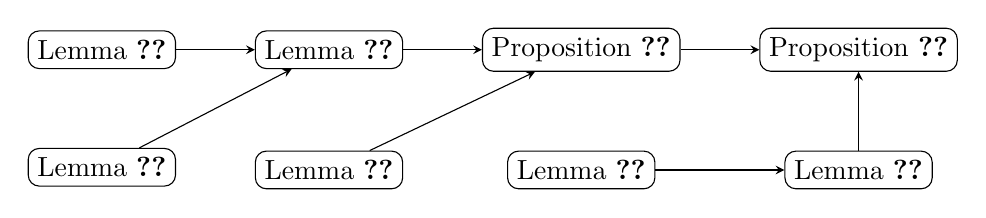
\begin{tikzpicture}[>=stealth,every node/.style={shape=rectangle,draw,rounded corners},]
\node (a1) {Lemma \ref{lem:transfer}};
\node (a2) [right =of a1] {Lemma \ref{lem:inverse}};
\node (a3) [below left =of a2] {Lemma \ref{lem:rot-inv}};
\node (a5) [right =of a2] {Proposition \ref{prop:prop1}};
\node (a4) [below left =of a5]{Lemma \ref{lem:ratio}};
\node (a6) [below =of a5] {Lemma \ref{lem:intertwin-pre}};
\node (a8) [right =of a5] {Proposition \ref{prop:prop2}};
\node (a7) [below =of a8] {Lemma \ref{lem:intertwin}};

\draw[->] (a1) to (a2);
\draw[->] (a3) to (a2);
\draw[->] (a2) to (a5);
\draw[->] (a4) to (a5);
\draw[->] (a6) to (a7);
\draw[->] (a5) to (a8);
\draw[->] (a7) to (a8);
\end{tikzpicture}
\caption{A diagram showing relations between assertions}\label{fig:diagram}
\end{center}
\end{figure*}

\vspace{1pc}


Step 3. \ We first recall the definition of $k_s$ given in \eqref{def-k_s}.  
 \begin{lemma}
 $k_s (x,y)$ is a positive definite kernel on $\mathbb R$. 
 \end{lemma}
 
 \begin{proof}
 For $r \in (0,1)$, let 
 \[ k^{(r)}_s (x,y) := \left(1-r \frac{(xy + 1)^2}{(x^2 + 1)(y^2 + 1)}\right)^{-s}. \]
 Since $(x,y) \mapsto \dfrac{1}{(x^2 + 1)(y^2 + 1)}$ and $(x,y) \mapsto (xy)^2 + 2xy + 1$ are both positive definite kernels on $\mathbb R$, 
 $(x,y) \mapsto \dfrac{(xy + 1)^2}{(x^2 + 1)(y^2 + 1)}$ is also a positive definite kernel on $\mathbb R$. 
 By the Taylor expansion, 
 $(1-x)^{-s} = \sum_{n=0}^{\infty} a_n x^n, \ |x| < 1$, 
 for $a_n \ge 0, n = 0,1, \cdots$. 
 Hence $ k^{(r)}_s (x,y)$ is a positive definite kernel on $\mathbb R$. 
 Since $$\lim_{r \to 1-0}  k^{(r)}_s (x,y) = k_s (x,y),$$
$ k_s (x,y)$ is also a positive definite kernel on $\mathbb R$. 
 \end{proof}

We second recall the definition of $\varphi_s$ given in \eqref{def-varphi_s}.  
By this and the quadrature rule for the Riemannian integral for continuous functions, 
it holds that for every $a < b$ and $r \in (0,1)$, 
 \[ \iint_{[a,b]^2} \frac{\varphi_s (x) \varphi_s (y) k^{(r)}_s (x,y)}{(x^2 + 1)(y^2 + 1)} dxdy \ge 0. \]
Since $0 \le k^{(r)}_s (x,y) \le k_s (x,y)$, 
 \[ \iint_{\mathbb R^2} \frac{   |\varphi_s (x) \varphi_s (y)|  k^{(r)}_s (x,y)}{(x^2 + 1)(y^2 + 1)} dxdy \]
 \[\le \iint_{\mathbb R^2} \frac{   |\varphi_s (x) \varphi_s (y)|  k_s (x,y)}{(x^2 + 1)(y^2 + 1)} dxdy \]
 \[\le \sum_{i.j=1}^{n} |c_i| |c_j| H_s (z_i, z_j) < + \infty.  \]
By the Lebesgue convergence theorem,  
we see that for every $r \in (0,1)$, 
 \[ \iint_{\mathbb R^2}  \frac{  \varphi_s (x) \varphi_s (y)  k^{(r)}_s (x,y)}{(x^2 + 1)(y^2 + 1)} dxdy \]
 \[= \lim_{n \to \infty} \iint_{[-n,n]^2} \frac{\varphi_s (x) \varphi_s (y) k^{(r)}_s (x,y)}{(x^2 + 1)(y^2 + 1)} dxdy \ge 0. \]
and furthermore, 
 \[ \iint_{\mathbb R^2}  \frac{  \varphi_s (x) \varphi_s (y)  k_s (x,y)}{(x^2 + 1)(y^2 + 1)} dxdy \]
 \[= \lim_{r \to 1-0} \iint_{\mathbb R^2}  \frac{  \varphi_s (x) \varphi_s (y)  k^{(r)}_s (x,y)}{(x^2 + 1)(y^2 + 1)} dxdy \ge 0. \]
This completes Step 3 and the proof.  
\end{proof}

\begin{remark}
It is easy to see that $H_{1/2} (z,w)$ is positive definite, because 
\[ H_{1/2} (z,w) = \int_{\mathbb R} \sqrt{p_{z}(x)} \sqrt{p_w (x)} dx. \]
See Remark \ref{rem:FH} (ii). 
\end{remark}

%%%
\section{$f$-divergences between the truncated Cauchy distribution}\label{sec:truncated}
%%%
 

Now we define the {\it truncated} distribution of univariate location-scale families. 
Let $p(x)$ be a positive Borel measurable function on $\mathbb{R}$ such that $\int_{\bbR} p(x) \dx = 1$. 
Let $M > 0$. 
Let 
\[ p^{\textup{t}}(x) := \begin{cases} c_M p(x) \ |x| \le M \\ 0 \ \ \ \  \ \ \ \  |x| > M \end{cases} \]
where $c_M := 1/\int_{-M}^{M} p(x) \dx$. 
For $l \in \mathbb{R}$ and $s > 0$, 
let 
\[ p^{\textup{t}}_{l,s}(x) := \frac{1}{s} p^{\textup{t}}\left(\frac{x-l}{s}\right).  \]

We consider the Kullback-Leibler divergence between truncated distributions.   
\begin{proposition}\label{proposition:KLD-truncated}
Assume that $p(x)$ is continuous on $\bbR$ and 
$-M s_2 + l_2 < -M s_1 + l_1 < M s_1 + l_1 < M s_2 + l_2$.
Then, 
$D_{\textup{KL}}(p^{\textup{t}}_{l_1,s_1}: p^{\textup{t}}_{l_2,s_2}) = +\infty$,  
and, 
$D_{\textup{KL}}(p^{\textup{t}}_{l_2,s_2}: p^{\textup{t}}_{l_1,s_1}) < +\infty.$
\end{proposition}

\begin{proof}
By the assumption, we have that 
$\{x : p^{\textup{t}}_{l_1, s_1}(x) > 0\} \subsetneq  \{x : p^{\textup{t}}_{l_2, s_2}(x) > 0\}$.  
Let  $U := \{x : p^{\textup{t}}_{l_2, s_2}(x) > 0 = p^{\textup{t}}_{l_1, s_1}(x) \}$. 
Then, 
\[ U = [-M s_2 + l_2, -M s_1 + l_1) \cup (M s_1 + l_1, M s_2 + l_2] \]
and  
\[ -\log \left(\frac{p^{\textup{t}}_{l_1, s_1}(x)}{p^{\textup{t}}_{l_2, s_2}(x)} \right) = +\infty \ \ x \in U. \]
Since $U$ has inner points, 
\[ \int_U -\log \left(\frac{p^{\textup{t}}_{l_1, s_1}(x)}{p^{\textup{t}}_{l_2, s_2}(x)} \right) p^{\textup{t}}_{l_2, s_2}(x) \dx = +\infty. \]
On the other hand, by the assumption that $p$ is continuous, 
$-\log \left(\frac{p^{\textup{t}}_{l_1, s_1}(x)}{p^{\textup{t}}_{l_2, s_2}(x)} \right) p^{\textup{t}}_{l_2, s_2}(x)$ is bounded on 
\[  \{x : p^{\textup{t}}_{l_2, s_2}(x) > 0\} \setminus U = \{x : p^{\textup{t}}_{l_1, s_1}(x) > 0\} \]
\[= [-M s_1 + l_1, M s_1 + l_1]. \]
Hence, 
\[ \int_{\{x : p^{\textup{t}}_{l_2, s_2}(x) > 0\} \setminus U}  -\log \left(\frac{p^{\textup{t}}_{l_1, s_1}(x)}{p^{\textup{t}}_{l_2, s_2}(x)}\right) p^{\textup{t}}_{l_2, s_2}(x) \dx < +\infty. \]
Hence, 
\[ D_{\textup{KL}}(p^{\textup{t}}_{l_1,s_1}: p^{\textup{t}}_{l_2,s_2}) \]
\[= \int_{\{x : p^{\textup{t}}_{l_2, s_2}(x) > 0\}}  -\log \left(\frac{p^{\textup{t}}_{l_1, s_1}(x)}{p^{\textup{t}}_{l_2, s_2}(x)}\right) p^{\textup{t}}_{l_2, s_2}(x) \dx = +\infty. \]

Since $-\log \left(\frac{p^{\textup{t}}_{l_2, s_2}(x)}{p^{\textup{t}}_{l_1, s_1}(x)} \right) p^{\textup{t}}_{l_1, s_1}(x)$ is bounded on 
$\{x : p^{\textup{t}}_{l_1, s_1}(x) > 0\} = [-M s_1 + l_1, M s_1 + l_1]$.
Hence, 
\[ D_{\textup{KL}}(p^{\textup{t}}_{l_2,s_2}: p^{\textup{t}}_{l_1,s_1}) \]
\[= \int_{\{x : p^{\textup{t}}_{l_1, s_1}(x) > 0\}}  -\log \left(\frac{p^{\textup{t}}_{l_2, s_2}(x)}{p^{\textup{t}}_{l_1, s_1}(x)}\right) p^{\textup{t}}_{l_1, s_1}(x) \dx < +\infty. \]
\end{proof}

The truncated Cauchy distribution and related issues have been investigated by many papers (e.g. \cite{Nadarajah2004, Nadarajah2007,  Ateya2013, Aldahlan2020}). 
Let $M > 0$. 
Let 
\[ p^{\textup{tc}}(x) := \begin{cases} \dfrac{c_M}{1+x^2} \ |x| \le M \\ 0 \ \ \ \   \ \  \ \ |x| > M \end{cases} \]
where $c_M := 2 \arctan(M)$. 
For $l \in \mathbb{R}$ and $s > 0$, 
let 
\[ p^{\textup{tc}}_{l,s}(x) := \frac{1}{s} p^{\textup{tc}}\left(\frac{x-l}{s}\right) =  \begin{cases} \dfrac{c_M s}{s^2+(x-l)^2} \ \  |x-l| \le Ms \\ 0 \ \ \  \ \ \ \ \ \ \  \ \ \ \ \ \ \  |x-l| > Ms \end{cases}.  \]
Contrarily to the Cauchy distribution, this distribution has moments of every order.

By Proposition \ref{proposition:KLD-truncated},  the Kullback-Leibler divergence between truncated Cauchy distributions can be infinite. 


\begin{proposition}
The Pearson chi-square divergence between the scale family of the truncated Cauchy distribution can be asymmetric. 
\end{proposition}

\begin{proof}
Let $M = 10$,  $(l_1, s_1) = (0,1)$ and $(l_2, s_2) = (0,2)$. 
Then, 
\[ D_\chi^P(p^{\textup{tc}}_{l_1, s_1}:p^{\textup{tc}}_{l_2, s_2}) =\int_{x : p^{\textup{tc}}_{l_1, s_1}(x) > 0} \frac{p^{\textup{tc}}_{l_2, s_2}(x)^2}{p^{\textup{tc}}_{l_1, s_1}(x)}\dx  -1 \]
\[= c_{10} \int_{-10}^{10} \frac{4(x^2 + 1)}{(x^2 + 4)^2} \dx -1, \]
and 
\[ D_\chi^P(p^{\textup{tc}}_{l_2, s_2}:p^{\textup{tc}}_{l_1, s_1}) =\int_{x : p_{l_2, s_2}(x) > 0} \frac{p^{\textup{tc}}_{l_1, s_1}(x)^2}{p^{\textup{tc}}_{l_2, s_2}(x)}\dx  -1 
\]
\[= c_{10} \int_{-20}^{20} \frac{(x^2 + 4) }{2(x^2 + 1)^2} 1_{|x| \le 10} \dx -1 \]
\[= c_{10} \int_{-10}^{10} \frac{(x^2 + 4) }{2(x^2 + 1)^2}  \dx -1. \]
We see that 
\[ \int_{-10}^{10} \frac{4(x^2 + 1)}{(x^2 + 4)^2} \dx = \frac{5}{52} (-3 + 26 \arctan(5)) \fallingdotseq 3.14504 \]
and 
\[ \int_{-10}^{10} \frac{x^2 + 4}{2(x^2 + 1)^2} \dx = \frac{15}{101} + \frac{5}{2} \arctan(10) \fallingdotseq 3.8263\]
Hence $D_\chi^P(p^{\textup{tc}}_{l_1, s_1}:p^{\textup{tc}}_{l_2, s_2}) \ne D_\chi^P(p^{\textup{tc}}_{l_2, s_2}:p^{\textup{tc}}_{l_1, s_1})$. 
\end{proof}

 

%%%%
\section{Code snippet for Taylor expansions of $f$-divergences}\label{sec:maximataylor}
%%%%%
We provide below a code using the {\sc Maxima}\footnote{\url{https://maxima.sourceforge.io/}} symbolic computing software to calculate the truncated Taylor series of $f$-divergences between two Cauchy distributions (instantiated for the Kullback-Leibler divergence).

{\scriptsize
\begin{verbatim}
Cauchy(x,l,s):=(s/(%pi*((x-l)**2+s**2)));
KLCauchy(l1,s1,l2,s2):=log(((s1+s2)**2+(l1-l2)**2)/(4*s1*s2));
l1:0;
s1:1;
l2:0.6;
s2:6/5;
k:40;
testcond: (9/16)-(l2**2+(s2-(4/5))**2);
print("Is condition>0 for Taylor expansion?:",testcond);
Cauchy1:Cauchy(x,l1,s1);
Cauchy2:Cauchy(x,l2,s2);
print("Exact KL");
KLCauchy(l1,s1,l2,s2);
ExactKL:float(%);
print("KL numerical integration:");
kla: quad_qagi( Cauchy1*log(Cauchy1/Cauchy2), x, minf, 
inf,'epsrel=1d-10); 
NumKL:float(kla[1]);

for i:2 while (i<=k)  
do( r[i]: quad_qagi( (Cauchy1-Cauchy2)**i/Cauchy2**(i-1), 
x, minf, inf,'epsrel=1d-10), print(i,r[i][1]));

print("KL Taylor truncated series:");
TaylorKL: sum( (((-1)**i)/i)*r[i][1], i, 2, k);
print("Exact:",ExactKL,"Numerical:",NumKL,
"Trunc.Taylor",TaylorKL);
print("Error |Taylor-Exact|",abs(TaylorKL-ExactKL));
\end{verbatim}
}


% you can choose not to have a title for an appendix
% if you want by leaving the argument blank
%\section{????}
%Appendix two text goes here.


% use section* for acknowledgment
\section*{Acknowledgment}


The authors would like to express their gratitude to two anonymous referees for many fruitful comments.  


% Can use something like this to put references on a page
% by themselves when using endfloat and the captionsoff option.
\ifCLASSOPTIONcaptionsoff
  \newpage
\fi



% trigger a \newpage just before the given reference
% number - used to balance the columns on the last page
% adjust value as needed - may need to be readjusted if
% the document is modified later
%\IEEEtriggeratref{8}
% The "triggered" command can be changed if desired:
%\IEEEtriggercmd{\enlargethispage{-5in}}

% references section

% can use a bibliography generated by BibTeX as a .bbl file
% BibTeX documentation can be easily obtained at:
% http://mirror.ctan.org/biblio/bibtex/contrib/doc/
% The IEEEtran BibTeX style support page is at:
% http://www.michaelshell.org/tex/ieeetran/bibtex/
%\bibliographystyle{IEEEtran}
% argument is your BibTeX string definitions and bibliography database(s)
%\bibliography{IEEEabrv,../bib/paper}
%
% <OR> manually copy in the resultant .bbl file
% set second argument of \begin to the number of references
% (used to reserve space for the reference number labels box)

\bibliography{fdivCauchy}
\bibliographystyle{IEEEtran}

%\begin{thebibliography}{1}

%\bibitem{IEEEhowto:kopka}
%H.~Kopka and P.~W. Daly, \emph{A Guide to \LaTeX}, 3rd~ed.\hskip 1em plus
%  0.5em minus 0.4em\relax Harlow, England: Addison-Wesley, 1999.

%\end{thebibliography}




% biography section
% 
% If you have an EPS/PDF photo (graphicx package needed) extra braces are
% needed around the contents of the optional argument to biography to prevent
% the LaTeX parser from getting confused when it sees the complicated
% \includegraphics command within an optional argument. (You could create
% your own custom macro containing the \includegraphics command to make things
% simpler here.)
%\begin{IEEEbiography}[{\includegraphics[width=1in,height=1.25in,clip,keepaspectratio]{mshell}}]{Michael Shell}
% or if you just want to reserve a space for a photo:

\begin{IEEEbiographynophoto}{Frank Nielsen}
%Biography text here.
Frank Nielsen was awarded his PhD on adaptive computational geometry (1996) from University of C\^ote d'Azur (France). 
He is a fellow of Sony Computer Science Laboratories Inc. (Japan) where he currently conducts research on 
the fundamentals and practice of geometric machine learning and intelligence with applications in visual computing. 
Frank Nielsen co-organizes with Fr\'ed\'eric Barbaresco the biannual conference Geometric Science of Information (GSI). 
\end{IEEEbiographynophoto}

% if you will not have a photo at all:
%\begin{IEEEbiographynophoto}{John Doe}
%Biography text here.
%\end{IEEEbiographynophoto}

% insert where needed to balance the two columns on the last page with
% biographies
%\newpage

\begin{IEEEbiographynophoto}{Kazuki Okamura}
Kazuki Okamura was awarded his PhD on mathematical sciences (2015) from the University of Tokyo (Japan). 
He is a lecturer in Department of Mathematics in Faculty of Science at Shizuoka University, Japan.
His research focuses mainly on probability theory and its applications.
%He is a member of the mathematical society of Japan. 
\end{IEEEbiographynophoto}

% You can push biographies down or up by placing
% a \vfill before or after them. The appropriate
% use of \vfill depends on what kind of text is
% on the last page and whether or not the columns
% are being equalized.

%\vfill

% Can be used to pull up biographies so that the bottom of the last one
% is flush with the other column.
%\enlargethispage{-5in}



% that's all folks
\end{document}


